%!TeX spellcheck = en-US

\RequirePackage{pdf14}
\documentclass[a4paper,11pt,twoside,openright]{thesis}
%\pdfminorversion=7

\usepackage{url}
\usepackage{amsmath}
\usepackage{color, graphicx, setspace}
\usepackage{subfigure}
\usepackage{amsmath, amsfonts}
\usepackage{lscape}
\usepackage{longtable}
\usepackage{quotchap}
\usepackage{csquotes}
\usepackage{tikz}
\usepackage{booktabs}
\usetikzlibrary{shapes,arrows}
\usetikzlibrary{calc}
\usetikzlibrary{fit,positioning}

\usepackage{algorithm}
\usepackage{algpseudocode}
%this is to fix nested function calls
\renewcommand*\Call[2]{\textproc{#1}(#2)}

\usepackage{colortbl}
\usepackage{xcolor}
\definecolor{pathwaynode}{RGB}{255,150,50}
\definecolor{independentnode}{RGB}{255,255,50}
\newcommand{\boz}{\cellcolor{pathwaynode}}
\newcommand{\ghool}{\cellcolor{independentnode}}


%\pdfoptionpdfminorversion 7
%\pdfpageattr {/Group << /S /Transparency /I true /CS /DeviceRGB>>}


\begin{document}
\frontmatter

\title{Interpretable Methods in Cancer Diagnostics}
\author{Adrin Jalali Khooshahr}
\date{2020}
\maketitle
%%% Information
\newpage{%
\null
\thispagestyle{empty}%
\begin{flushright}
\null
\begin{table}[b!]
  \centering
  \begin{tabular}[b]{l|l}
    \textbf{Day of colloquium}         & \\%20.12.2019\\[1.1em]
    \textbf{Dean of the faculty}       & \\%Univ.-Professor Dr. Sebastian Hack\\[1.1em]
    \\
    \textbf{Chair of the committee}    & \\%Prof.~Dr. Volkhard Helms\\[1.1em]
    \textbf{Reporters} & \\
    \textbf{First Reviewer}            & \\%Prof.~Dr.~Nico Pfeifer\\%[1.1em]
    \textbf{Second Reviewer}           & \\%Prof.~Dr.~Olga Kalinina\\%[1.1em]
    \textbf{External Reviewer}         & \\%Dr. Ryan Brinkman\\
    \textbf{Academic assistant}        & \\%Dr.~
  \end{tabular}
\end{table}
\null
\end{flushright}
\newpage}
\newpage{%
\null
\thispagestyle{empty}%
\newpage}
%%% Dedication
\newpage{%
\null
\thispagestyle{empty}%
\begin{flushright}
\null\vspace{\stretch{3}} 
\textit{To Aleks}
\vspace{\stretch{5}}\null
\end{flushright}
\newpage}
\newpage{%
\null
\thispagestyle{empty}%
\newpage}
% Adjust page numbers
\addtocounter{page}{-6}%

\chapter*{Acknowledgment}
This thesis would not have been possible without the help and support of many
individuals, collaborators, and my supervisors. I deeply appreciate their help
and acknowledge I would not have been able to finish this work without their
help.

First and foremost, I am grateful of the support I received from my supervisors
Prof. Dr. Nico Pfeifer and Prof. Dr. Dr. Thomas Lengauer at the Max Planck
Institute for Informatics in Saarbr\"ucken, Germany, and Dr. Ryan Brinkman at
the Terry Fox Labs in the British Columbia Cancer Research Center in Vancouver,
Canada. I also would like to thank Dr. MD. Andrew Weng in the same lab.

I am also extremely thankful of my partner Aleksandra Piwowarek and my parents
who have been very supportive and encouraging during the hard times and never
gave up on being encouraging. I would not have finished this thesis without
their continuous support.

I would like to extend this acknowledgment to my colleagues with whom I have
worked and collaborated, and who have supported me with all the brainstorming
and discussions we have had. The list is long, but I would like to mention
Sarvesh Nikumbh, Nora Speicher, Anna Feldmann, Nima Aghaeepour, and Kieran
O'Neil.

The last, but not least, is to acknowledge the support I have received from my
friends from all around the world. I would like to mention Marjan Farahbod,
Iran Mansoori, Matti Lyra, Hassan Hatefi, Faraz Makari, Rob McGee, and Cyrus
Altschuck.

\begin{abstract}
Cancer is a hard problem. It is hard for the patients, for the doctors and
nurses, and for the researchers working on understanding the disease and
finding better treatments for it. The challenges faced by a pathologist
diagnosing the disease for a patient is not necessarily the same as the ones
faced by cell biologists working on experimental treatments and understanding
the fundamentals of cancer. In this thesis we work on different challenges
faced by both of the above teams.

This thesis first presents methods to improve the analysis of the flow
cytometry data used frequently in the diagnosis process, specifically for the
two subtypes of non-Hodgkin Lymphoma which are our focus: Follicular Lymphoma
and Diffuse Large B Cell Lymphoma. With a combination of concepts from graph
theory, dynamic programming, and machine learning, we present methods to
improve the diagnosis process and the analysis of the abovementioned data. The
interpretability of the method helps a pathologist to better understand a
patient's disease, which itself improves their choices for a treatment.

In the second part, we focus on the analysis of DNA-methylation and gene
expression data, both of which presenting the challenge of being very high
dimensional yet with a few number of samples comparatively. We present an
ensemble model which adapts to different patterns seen in each given data, in
order to adapt to noise and batch effects. At the same time, the
interpretability of our model helps a pathologist to better find and tune the
treatment for the patient: a step further towards personalized medicine.
\end{abstract}

\selectlanguage{ngerman}%
\begin{abstract}
Krebs ist ein schweres Problem. Es ist schwer für die Patienten, für die Ärzte
und Krankenschwestern und für die Forscher, die daran arbeiten, die Krankheit
zu verstehen und eine bessere Behandlung dafür zu finden. Die
Herausforderungen, mit denen ein Pathologe konfrontiert ist, um die Krankheit
eines Patienten zu diagnostizieren, müssen nicht die gleichen sein, mit denen
Zellbiologen konfrontiert sind, die an experimentellen Behandlungen arbeiten
und die Grundlagen von Krebs verstehen. In dieser Arbeit beschäftigen wir uns
mit verschiedenen Herausforderungen, denen sich beide oben genannten Teams
stellen.

In dieser Arbeit werden zunächst Methoden vorgestellt, um die Analyse der im
Diagnoseverfahren häufig verwendeten Durchflusszytometriedaten zu verbessern,
insbesondere für die beiden Subtypen des Non-Hodgkin-Lymphoms, auf die wir uns
konzentrieren: das follikuläre Lymphom und das diffuse großzellige
B-Zell-Lymphom. Mit einer Kombination von Konzepten aus Graphentheorie,
dynamischer Programmierung und maschinellem Lernen präsentieren wir Methoden
zur Verbesserung des Diagnoseprozesses und der Analyse der oben genannten
Daten. Die Interpretierbarkeit der Methode hilft einem Pathologen, die
Apatientenkrankheit besser zu verstehen, was wiederum seine Wahlmöglichkeiten
für eine Behandlung verbessert.

Im zweiten Teil konzentrieren wir uns auf die Analyse von DNA-Methylierungs-
und Genexpressionsdaten, die beide die Herausforderung darstellen, sehr
hochdimensional zu sein, jedoch mit nur wenigen Proben im Vergleich. Wir
präsentieren ein Zusammenstellungsmodell, das sich an unterschiedliche Muster
anpasst, die in den jeweiligen Daten zu sehen sind, um sich an Rauschen und
Batch-Effekte anzupassen. Gleichzeitig hilft die Interpretierbarkeit unseres
Modells einem Pathologen, die Behandlung für den Patienten besser zu finden und
abzustimmen: ein Schritt weiter in Richtung personalisierter Medizin.
\end{abstract}
\selectlanguage{english}%

\tableofcontents

\mainmatter


\begin{savequote}[.5\linewidth]
  ``Growth for the sake of growth is the ideology of the cancer cell.''
  \qauthor{- Edward Abbey}
\end{savequote}
\chapter{Introduction}
\label{ch:intro}
Cancer has been with human species throughout our 4000 years of history.
Although our understanding of cancer has changed drastically through time, its
treatment stays challenging and in many cases we have not been able to cure it
to this date. The immense frustration of dealing with cancer not only affects
the patients, but also the doctors, pathologists, and oncologists treating
those patients. Siddhartha Mukherjee in his book ``The Emperor of All
Maladies'' explains the feeling with these
words~\cite[prologue]{the-emperor-of-all-maladies}:

\begin{displayquote}
  ...
  
  There were seven such cancer fellows at this hospital. On paper, we seemed
  like a formidable force: graduates of five medical schools and four teaching
  hospitals, sixty-six years of medical and scientific training, and twelve
  postgraduate degrees among us. But none of those years or degrees could
  possibly have prepared us for this training program. Medical school,
  internship, and residency had been physically and emotionally grueling, but
  the first months of the fellowship flicked away those memories as if all of
  that had been child's play, the kindergarten of medical training.

  ...

  The stories of my patients consumed me, and the decisions that I made haunted
  me. \emph{Was it worthwhile continuing yet another round of chemotherapy on a
    sixty-six-year-old pharmacist with lung cancer who had failed all other
    drugs? Was it better to try a tested and potent combination of drugs on a
    twenty-six-year-old woman with Hodgkin's disease and risk losing her
    fertility, or to choose a more experimental combination that might spare
    it? Should a Spanish-speaking mother of three with colon cancer be enrolled
    in a new clinical trial when she can barely read the formal and inscrutable
    language of the consent forms?}
\end{displayquote}

I can better put this thesis in context by giving my personal perspective on
cancer research and diagnosis. I spent over a year researching in British
Columbia's Cancer Research Center (BCCRC) in Vancouver, Canada, which also
admitted patients for diagnosis and treatment. As a result, I worked closely
with oncologists who were diagnosing patients as well as cell biologists
researching fundamentals of cancer. Their experiences and the challenges they
were facing had a great impact on me and to a large extent shaped my research
for the next few following years. Then, once I moved to the Bioinformatics lab
in Max Planck Institute for Informatics in Saarbr\"ucken, Germany, I was better
equipped with required statistics and machine learning skills to tackle the
computational problems explained here. Following are a few examples of
challenges I saw people were facing in BCCRC:

\begin{itemize}
  \item Some patients enter the clinic carrying cancer type A, which is mild
    and does not require an aggressive treatment. Therefore they are put under
    the appropriate treatment while their condition is monitored through time.
    However, the disease in some of these patients develops into another type,
    let say type B, which is more aggressive and sometimes requires a harsher
    or a different treatment. Considering the fact that like many other
    diseases, cancer can be defeated best in its earliest stages, we could
    potentially achieve a better prognosis for these patients had we known
    their disease will develop into type B at a much earlier stage.

  \item Similar to the above issue, out of the many patients who go in
    remission, \emph{i.e} they seem free of cancer after the course of the
    treatment, some relapse with a cancer which is significantly more resistant
    to usual treatments compared to when they where originally diagnosed. This
    sometimes happens when a very small number of cells from the original
    cancer are or become resistant to the drugs and survive the treatment, but
    go undetected for a while in the tests and scans. It may take months for
    them to grow large enough to be detected again. Now the question is,
    looking back at the data of these patients, could we detect those cells, or
    something about the original cancer cells predicting the relapse, earlier
    during the treatment or even at the time of the original diagnosis?

  \item In BCCRC, people were also researching cancer by looking at the effects
    of different drugs and drug combinations targeting different genes. Some of
    my cell biologist friends, often taking recommendations from their
    supervisors, would choose a few genes and spend years investigating the
    role of those genes in the development of a particular cancer type. Of
    course they would do their best to choose the most relevant set of genes to
    their knowledge, but the task of choosing a few genes out of over 22k genes
    on the human genome is rather challenging and does not always lead to
    positive results and successful treatments. There is also a bias towards
    the genes which have been discovered earlier and have been studied more in
    depth. If the cancer happens to be related to one of the less studied
    genes, it usually can stay under the radar for while.
\end{itemize}

TODO: The two parts are not clear

These(TODO: ?) decisions are hard to make, and it does not help knowing that
our deep understanding of cancer is far from complete. The battle against
cancer has many fronts, including prevention, diagnosis, and treatment, all of
which benefiting from the advancements in understanding the disease. As a part
of the process, cancer researchers try to understand the disease in the lab,
and once their findings are confirmed, accepted by the community, and pass the
legal requirements, they are used by pathologists and oncologists in the
clinics. However, the diagnosis itself is also complex, challenging, and in
many cases not a definitive one. This is why sometimes doctors do not agree on
the exact diagnosis, and a counsel of experts is required for a better and more
reliable diagnosis and a treatment which hopefully results in a better
prognosis.

Cancer is a collection of extremely smart and complicated diseases. Although
they share many common characteristics, the same treatment does not result in a
similar prognosis. For example, two patients may come with two very similar
malignant tumors in their breasts. However, one of the patient's tumor grows in
response to estrogen, while the other one shows no reaction to estrogen. In
this case, a treatment which blocks estrogen receptors is very effective for
the first patient (ER+), while being completely ineffective against the second
patient who has an ER- subtype of breast cancer.

At the core of it, it comes to the fact that in normal cells there are
processes and checks put in place which define when and if the cell should
divide or die at a certain time or under certain conditions. Some of those
mechanisms act like an automated self destruct switch which is triggered if
something goes wrong in the cell. However, our cells are under constant stress
from the external factors which damage them, UV being one example, and
sometimes the damage to the cell affects those mentioned mechanisms and
disables them. This may lead the cell to divide uncontrollably, and become
cancerous. Another difference between normal cells and cancerous ones, is that
normal cells are capable of repairing most of the mutations happening on their
DNA, whereas those processes themselves are damaged in a cancerous cell. As a
result, the rate of mutation in cancerous cells is higher of a few orders of
magnitude compared to a normal healthy cell. The high rate of cell division in
combination with hyper mutation, makes cancerous cells very adaptive to their
environment, as well as against the drugs attacking them.

Cancer treatments are methods and substances which ideally target only the
cancerous cells and kill them. In a sense, they are poison, but ideally only to
cancer. However, cancer cells are derived from our own cells, and therefore it
is not easy to distinguish them from normal cells. The more difference between
the cancer cells and our normal healthy cells, the easier to target them; but
unfortunately not all cancer subtypes are easily distinguishable from other
cells for the purpose of treatment.

TODO: we don't say why we help and how

This thesis is an effort to design and develop computational methods to tackle
the abovementioned challenges. There are two main parts to this thesis. In the
first part, presented in Chapter~\ref{sec:fcs}, the focus is mostly on the
methods applicable directly in clinics, using the kind of data readily
available at the time of the diagnosis. The technology required to produce the
required data is not new and it has been in widespread use for decades all
around the world. The technology is called flow cytometry and the machine
producing the data is a flow cytometer. The machine takes certain measurements
from single cells, one by one, allowing us to study the presence and absence of
certain cell types in a single biopsy. It also allows us to sort and extract
certain cell types from the biopsy for further analysis on only those selected
cells. Although the technology has been around for a while, up until recently
researchers have been analyzing its data manually. This work presents methods
to automate some of those laborious and tedious tasks, while deriving new
information and insights about the data at the same time. As a byproduct, these
methods can be used to design tests which can be run on cheaper machines
available in poorer countries using the data from the more advanced machines,
and yet deliver a relatively similar performance.

TODO: chapter 3 doesn't seem new here.

TODO: be clear on what is done!

TODO: same paragraph as above

More specifically, one way pathologists study a given biopsy, is to find out
what kinds of cells are present in a given sample, and what types of
irregularities they posses. Each of these groups of cells is called a cell
population, and what is presented in Chapter~\ref{sec:fcs} is an effort to find
different ways of discovering meaningful cell populations in each given sample.
At the same time, we detect certain cell populations which appear to be
correlated with a specific disease, or are helpful differentiating between
two subtypes of a disease.

The other part of this thesis is closer to the bleeding edge of cancer research
compared to what happens in clinics. It uses some types of data, such as gene
expression profiles and DNA methylation data, which are more expensive to
acquire and are usually measured for the purpose of research. A gene expression
profile measures the activity of all 22k+ genes in a given sample, and a usual
DNA methylation profile measures the methylation level of about 450k sites on
the human DNA. These data, as well as others such as DNA, RNA, and protein
sequence data have been increasingly used by biologists and computational
biologists to better understand cell biology in many fields, including cancer
research. These data and methods have been so essential to our understanding of
cancer that the classification of some cancer types now depend on them. In some
cases, they(?, TODO) have shown us that two different classes of cancer are
indeed the same disease, only in different stages. Lymphoma and leukemia are
two good examples which used to be considered two different cancers, and now
put together in the \emph{lymphoid neoplasms} group.

TODO: bad place, move up?

TODO: what's the other one?

One goal of this thesis is to design computational methods capable of reporting
a list of promising genes that are influential in determining the cancer
subtypes, so that the same set of genes can be a better starting point for cell
biologists to choose and investigate. Doing so, we can also deliver a list of
genes specific to each patient, enabling the selection of a rather personalized
treatment for the patient.

Although there has been magnificent advancements in the field from the
computational perspective, these(?, TODO) are very hard problems. The curse of
dimensionality on top of the low number of samples compared to the number of
dimension in the data all result in a hard computational problem as further
explained in Section~\ref{sec:background}). Also, the fact that the data is
often affected by noise and batch effects doesn't help the case neither, which
we cover in more detail in Section~\ref{sec:adaptive-learning}. Another
challenging factor is that cancer, and even a single cancer tumor, is
heterogeneous and different cases show very different varying genetic profiles.
Historically this has lead to further classification of cancer, and at times,
changing the classification and merging some classes all together as mentioned
above.

All of the above facts and arguments motivated me to focus on investigating
interpretable machine learning models so that:
\begin{itemize}
\item The result of the investigation and application of the model on the data
  results in better understanding of the disease, by giving cell biologists
  hints about where they can put their focus.
\item For any given data from a single patient, the model can give some
  information about the potential underlying cause of the disease which in
  combination with the fact that we often times have several treatment options
  for the same disease can be used in the diagnosis phase to improve the
  treatment and prognosis. (TODO: one sentence!)
\item For a trained model, give an overall explanation on how the model is
  working so that it can better be trusted and understood by the people in
  clinics.
\end{itemize}

In the following chapters, some of the basics required to follow the later
sections, covering some background in the related parts of machine learning and
biology are covered in chapter~\ref{sec:background}. In chapter~\ref{sec:fcs}
we focus on flow cytometry data and explain the design and implementation of a
few pieces which together make an end to end pipeline to analyze such data, and
apply that to some specific lymphoma subtypes. Then we continue in
chapter~\ref{sec:adaptive-learning} with the analysis of mostly DNA methylation
data and design some adaptable and interpretable models with an eye on
personalized medicine.

TODO: what are the concrete research questions?


\chapter{Background}
\label{sec:background}

\section{Machine Learning}
Machine learning techniques are used to extract information from data, or make some predictions about the data. This chapter briefly explains methods and techniques used in, or required to understand the proceeding chapters.

We can recognize two groups of learning problems: supervised and unsupervised learning. Supervised learning deals with data sets that are in the form of a set of input and outputs, and the task at hand is to predict the output using the input~\cite[Ch. 2]{statistical-learning},~\cite[Ch. 1]{murphy2012machine}. Classification and regression are supervised learning problems. Unsupervised learning, on the contrary, deals with data sets which are in the form of a set of data points, and no output is given. Clustering the most studied unsupervised learning problem~\cite[Ch. 14]{statistical-learning}~\cite[Ch. 1]{murphy2012machine}.

\subsection{Empirical Risk Minimization}
\label{chap:empirical-risk-minimization}
As mentioned above, supervised learning deals with predicting an output $y_i \in Y$ given an input $x_i \in X$. The task is to find a function $f(.)$ which best predicts the output, given any possible input. Because in practice we have access to a limited given data set, the best we can do is to find a function that best predicts the output given any input in the data set.

We can formulate finding the best function $f(.)$, as finding a function that has the minimum loss over the data. Therefore we need a loss function which is defined as $L(x, y, f(x))$, with $x$ the input, $y$ the desired output, and $f(x)$ the predicted output. The loss value has to be in $[0, \infty)$, and $L(x, y, y) = 0$~\cite[p. 62]{learning-with-kernels}. The empirical risk function is then defined as~\cite[p. 67]{learning-with-kernels}:

  \begin{align}
    R_{emp}[f] := \frac{1}{m}\sum_{i = 1}^{m} L(x_i, y_i, f(x_i))
  \end{align}
  
Now let $\mathcal{F}$ be the function space available to choose $f(.)$ from it. The best function is one which minimizes the risk function~\cite[p. 67]{learning-with-kernels}:

\begin{align}
  \arg \min_{f \in \mathcal{F}} R_{emp}[f] = \arg \min_{f \in \mathcal{F}} \frac{1}{m}\sum_{i = 1}^{m} L(x_i, y_i, f(x_i))
\end{align}

But there is a problem with the above formulation, if the function space $\mathcal{F}$ is rich enough to fit to the given data too well. Imagine a function that returns $y_i$ for each $x_i$ in the training set, and $0$ otherwise. This function clearly has a minimum loss of $0$, but does not generalize on unseen data. This is called overfitting in machine learning. One way to fix this issue is to regularize the loss function in some way, and give preference to functions $f(.)$ with lower complexity, or smoother functions. This is referred to as regularized empirical risk minimization~\cite[Ch. 4.1]{learning-with-kernels}, or structural risk minimization~\cite[Ch. 4.1]{thenatureofstatisticallearningtheory}. Assume $\Omega(f)$ is a penalty assigned to function $f(.)$; then the regularized empirical risk is formulated as:

\begin{align}
  R_{emp}[f] := \frac{1}{m}\sum_{i = 1}^{m} L(x_i, y_i, f(x_i)) + \lambda \Omega(f)
  \label{frm:bkg:emp-regularized}
\end{align}

Parameter $\lambda$ is the regularization term and we estimate it, among other among other parameters, using cross validation.

\subsection{Cross Validation}
\label{chap:cross-validation}

Cross validation is a technique used in method selection and performance estimation. In cross validation we divide the given training data into $k$ folds, set aside one of those $k$ folds, train the model on $k - 1$ remaining sections, and test the performance of the model on the set aside part of the data. Then repeat this process for all $k$ folds to assess the overall performance of the method. A special case of $k$-fold cross validation is leave-one-out in which $k=n$, the number of samples. Leave-one-out cross validation is computationally intensive for relatively large number of samples. A popular $k$ is 10, which is shown to have lower variance than leave-one-out method, and it has a low bias~\cite[Ch. 7]{statistical-learning}. 

There are also some variations to the simple $k$-fold cross validation scheme. One way is to repeat the $k$-fold system multiple times with a random shuffle of the data before each $k$-fold test, and calculate the estimated error using the repeated test. Another variation is to randomly partition the data into train and test partitions several times and use these sets to estimate the performance of the method.

The latter two variations are shown to give better estimates of the true error of the method compared to bootstrap and a single $10$-fold scheme~\cite{kim2009estimating, efron1994introduction}. Because repeating a $k$-fold scheme can be computationally intensive depending on the method being tested, we sometimes use a repeated random partitioning of the data in our work. In some even more computationally intensive cases, we have limited our analysis to a single $k$-fold to select methods.
  
\subsection{Feature Selection}
Feature selection is the task of selecting important features to the problem at hand. It becomes particularly a hard task when the number of features in the data is of a higher magnitude compared to the number of given samples. Table~\ref{tab:sample-sample-size} shows an example number of samples vs. number of features in a typical data. One of the challenges when dealing with such a large number of features is that if enough number of features have a probability distribution independent of the outcome, some of them might falsely seem correlated with the outcome. Another obstacle comes from the fact that our features are not independent and they function in complex networks. As a result, features should be considered in groups, which is a combinatorial and intractable problem.

\begin{table}[th!]
  \centering
  \begin{tabular}{p{.2\textwidth} p{.3\textwidth} p{.38\textwidth}}
    \hline
    \multicolumn{3}{c}{Sample Data} \\
    \cline{1-3}
    Sample Count   & Gene Expression Data Feature Count & 450K Methylation Chip Data Feature Count \\
    \hline
    $500$      & $\approx 20,000$    & $\approx 450,000$   \\
    \hline
  \end{tabular}
  \caption{An example number of samples and features in our usual data}
  \label{tab:sample-sample-size}
\end{table}

We have used correlation~\cite{correlation}, mutual information~\cite{mutual-information}, and $l_1$-regularized methods~\cite{l1-regularized} as techniques to select features.

\subsection{Classification}
Classification is the problem of putting data into different classes~\cite[Ch. 1]{statistical-learning}. During the training phase, the matrix $X_{samples \times features}$ is given as the input and $y_{samples}$ as the desired output. The vector $y$ has values from a discrete set. If the set has only two distinct values, the problem is called a binary classification.

Logistic regression~\cite{logistic-regression1,logistic-regression2}, Support Vector Machines (SVM)~\cite{svm1,svm2}, and decision trees~\cite[Ch. 9]{statistical-learning} are examples of classification methods.

\subsection{Regression}
In statistics, predicting a continues output value given an input data is called regression~\cite[Ch. 1]{statistical-learning}. Regression and classification differ in their desired output type. In regression the output is continues in contrast to classification in which the output is a discrete value.

Linear regression~\cite[Ch. 3]{statistical-learning}, Gaussian processes~\cite{gaussian-processes}, and kernel based regression~\cite[Ch. 9]{learning-with-kernels} are some available methods here.

\subsection{Regularization}
Building a machine to predict the outcome with a good performance on the training set is easy if the number of features in the data is large enough compared to the number of samples, even if features are drawn from a random background probability distribution independent of the outcome. But the trained machine will perform poorly on the unseen test samples. This phenomenon is called overfitting. One way to prevent overfitting is to select potential features before training a selected model.

Another way to tackle the problem is to reduce the complexity of the models. This can be done via regularization. The $l_1$-regularization is an appropriate tool when the intention is to reduce the number of features a model takes into account for prediction as well as its complexity~\cite{l1-regularized}.

Assume a model minimizes a loss function $E(X, Y)$, where $X$ is the input matrix and $Y$ is the output vector or matrix. In most regression models the loss function is defined as:

\begin{align}
  E(X, Y) = \parallel Y - X \beta \parallel_2
  \label{frm:loss-function}
\end{align}

The optimization algorithm finds a $\beta$ that minimizes the loss function in Formula~\ref{frm:loss-function}. Having enough number of features, the optimization algorithm might find a $\beta$ that gives a perfect loss, i.e. 0. But in noisy environments the resulting $\beta$ is probably not the real $\beta$ of the underlying model producing the data. The vector $\beta$ might also have some extreme values that are likely not desired. Penalizing the \emph{size} of $\beta$ as shown in Formula~\ref{frm:regularized} will address the abovementioned concern. The size of a vector in this context is represented by its $l_1$ or $l_2$ norm as defined in Formula~\ref{frm:lp-norm}.


\begin{align}
  \parallel \beta \parallel_p := \left(\sum\limits_{i=1}^n \mid \beta_i \mid^p \right)^{1/p}
  \label{frm:lp-norm}
\end{align}
\begin{align}
  &E(X, Y) + \alpha \parallel \beta \parallel_2 = \parallel Y - X \beta \parallel_2 + \alpha \parallel \beta \parallel_2 \nonumber \\
  &\text{or} \nonumber \\
  &E(X, Y) + \alpha \parallel \beta \parallel_1 = \parallel Y - X \beta \parallel_2 + \alpha \parallel \beta \parallel_1
  \label{frm:regularized}
\end{align}

\subsection{Support Vector Machines}
\label{sec:svms}

Support vector machines (SVM) can be used both for regression and classification tasks~\cite{svm2, svr1}. As a classifier, SVM finds an optimal hyperplane to separate data points in the feature space by maximizing the hyperplane's margin to the nearest point. Therefore given a test data point, its side with regard to the hyperplane determines its class. As a regressor however, SVM finds an optimal hyperplane to interpolate given data points by minimizing the hyperplane's distance from data points.

Formally speaking, given data-set $\mathcal{D}$ of $n$ data points:

\begin{align}
  \mathcal{D}={(\mathbf{x}_i, y_i) | \mathbf{x}_i \in \mathbb{R}^p, y_i \in {-1, 1}}_{i=1}^{n}
\end{align}

where $\mathbf{x}_i$ is a real vector of length $p$, and $y_i$ is either $1$ or $-1$. A $p$-dimensional hyperplane, characterized by its normal vector $\mathbf{w}$ and its intercept $\mathbf{b}$, is the set of points $\mathbf{x}$ that fit in Formula~\ref{frm:hyperplane}.

\begin{align}
  \mathbf{w} . \mathbf{x} - b = 0
  \label{frm:hyperplane}
\end{align}

Now consider two hyperplanes on both sides of the abovementioned hyperplane as formulated bellow:

\begin{align}
  \mathbf{w} . \mathbf{x} - b &= 1 \nonumber \\
  \mathbf{w} . \mathbf{x} - b &= -1
\end{align}

The distance between each of these hyperplanes and the on in the middle is $\frac{1}{\parallel \mathbf{w} \parallel}$. Therefore the distance between the two of them is $\frac{2}{\parallel \mathbf{w} \parallel}$. For now we assume the data is linearly separable in its feature space, i.e. there exists a hyperplane that separates the data into two classes without error. Such a hyperplane satisfies the following constraint:

\begin{align}
  y_i (\mathbf{w} . \mathbf{x}_i - b)\geq 1 \text{ for all } 1 \leq i \leq n
\end{align}

An optimal hyperplane is one such that it maximizes the margin; hence formulated as Formula~\ref{frm:svm2}. An illustration of the optimal solution is presented in Fig.~\ref{fig:svm-hyperplane}.

\begin{align}
  &\arg\max_{(\mathbf{w},b)}\frac{1}{\|\mathbf{w}\|_2} \nonumber \\
  &\text{s.t.} \nonumber \\
  &y_i (\mathbf{w} . \mathbf{x}_i - b)\geq 1 \text{ for all } 1 \leq i \leq n
  \label{frm:svm2}
\end{align}

\begin{figure}[!ht]
  \centering
  \includegraphics[width=.5\textwidth]{figs/background/Svm_max_sep_hyperplane_with_margin}
  \caption{Illustration of the optimal hyperplane in a support vector machine model, for a 2-dimensional data.}
  \label{fig:svm-hyperplane}
\end{figure}

However, for an easier optimization and mathematical convenience, the above optimization problem is usually formulated as Formula~\ref{frm:svm1} which has the same solution as $\mathbf{w}$ and $b$~\cite[Ch. 5]{thenatureofstatisticallearningtheory},~\cite[Ch. 7]{learning-with-kernels}.

\begin{align}
  &\arg\min_{(\mathbf{w},b)}\frac{1}{2}\|\mathbf{w}\|_2^2 \nonumber \\
  &\text{s.t.} \nonumber \\
  &y_i (\mathbf{w} . \mathbf{x}_i - b)\geq 1 \text{ for all } 1 \leq i \leq n
  \label{frm:svm1}
\end{align}

which can be written as Formula~\ref{frm:svm3} after introducing Karush-Kuhn-Tucker (KKT) multipliers~\cite{kkt-orig}~\cite[Ch. 5]{thenatureofstatisticallearningtheory}.

\begin{align}
  &\arg\min_{\mathbf{w},b } \max_{\boldsymbol{\alpha}} \left\{ \frac{1}{2}\|\mathbf{w}\|_2^2 - \sum_{i=1}^{n}{\alpha_i[y_i(\mathbf{w}\cdot \mathbf{x_i} - b)-1]} \right\} \nonumber \\
  &\text{s.t.} \nonumber \\
  &\alpha_i \geq 0 \text{ for } 1 \leq i \leq n \nonumber \\
  \label{frm:svm3}
\end{align}

Multipliers $\alpha_i$ will be $0$ for each $\mathbf{x}_i$ that does not lie on either of the marginal hyperplanes. For example in Figure~\ref{fig:svm-hyperplane}, $\alpha_i$ is non-zero for only three of the data points; the ones that are exactly on either of the marginal lines. The corresponding $\mathbf{x}_i$ for which $\alpha_i$ is non-zero, are \emph{support vectors}.

It can be shown that Formula~\ref{frm:svm-dual1} is a dual of the optimization problem defined in Formula~\ref{frm:svm3}~\cite[p. 14]{learning-with-kernels}~\cite[Ch. 5]{thenatureofstatisticallearningtheory}.

\begin{align}
  &\arg\max_{\boldsymbol{\alpha}}\left\{\sum_{i=1}^n \alpha_i - \frac{1}{2}\sum_{i, j} \alpha_i \alpha_j y_i y_j \mathbf{x}_i^T \mathbf{x}_j\right\} \nonumber \\
  &\text{s.t.} \nonumber \\
  &\alpha_i \geq 0 \text{ for } 1 \leq i \leq n \nonumber \\
  &\sum_{i=1}^{n}\alpha_i y_i = 0
  \label{frm:svm-dual1}
\end{align}

Now assume the following notations and definitions:

\begin{align}
  \phi(\mathbf{x}) &:= \mathbf{x} \nonumber \\
  \langle \mathbf{x}_i, \mathbf{x}_j \rangle &:= \mathbf{x}_i^T \mathbf{x}_j \nonumber \\
  k(\mathbf{x}_i, \mathbf{x}_j) &:= \langle \phi(\mathbf{x}_i), \phi(\mathbf{x}_j) \rangle
  \label{frm:svm-ktrick1}
\end{align}

Putting function $k$ in Formula~\ref{frm:svm-dual1}, the SVM's optimization problem can be written as:

\begin{align}
  &\arg\max_{\boldsymbol{\alpha}}\left\{\sum_{i=1}^n \alpha_i - \frac{1}{2}\sum_{i, j} \alpha_i \alpha_j y_i y_j k(\mathbf{x}_i, \mathbf{x}_j)\right\} \nonumber \\
  &\text{s.t.} \nonumber \\
  &\alpha_i \geq 0 \text{ for } 1 \leq i \leq n \nonumber \\
  &\sum_{i=1}^{n}\alpha_i y_i = 0
  \label{frm:svm-dual2}
\end{align}

The identity function used in Formula~\ref{frm:svm-ktrick1} is not the only option. We can transform the data into another feature space using a different $\phi(.)$, and then use dot-product in that space. This is useful for cases that the data is not linearly separable in its original feature space, but linearly separable using a non-linear transformation.

Using Mercer's theorem~\cite{mercer-theorem} and its corollary Mercer's condition, it can be shown that any function $k$ satisfying the following condition can be used as a \emph{kernel} in Formula~\ref{frm:svm-dual2}~\cite[Ch. 2.2]{learning-with-kernels}.

\begin{align}
  \forall \mathcal{D}, \forall c_i, c_j \in \mathbb{R}: \sum_{i=1}^n\sum_{j=1}^n k(\mathbf{x}_i, \mathbf{x}_j) c_i c_j \geq 0
  \label{frm:positive-definite}
\end{align}

Arguably, other than dot-product, the most famous kernel function $k$ satisfying the above condition is the \emph{Gaussian kernel}, also known as the \emph{radial basis function (RBF) kernel}~\cite[Ch. 2]{learning-with-kernels}:

\begin{align}
  &k(\mathbf{x_i}, \mathbf{x_j}) = \exp\left(-\frac{||\mathbf{x_i} - \mathbf{x_j}||^2}{2\sigma^2}\right) \nonumber \\
  &\sigma \in \mathbb{R}
  \label{frm:rbf-kernel1}
\end{align}

Many implementations use a different formulation which uses a different parametrization, using $\gamma=\frac{1}{2\sigma^2}$:

\begin{align}
  &k(\mathbf{x_i}, \mathbf{x_j}) = \exp\left(-\gamma||\mathbf{x_i} - \mathbf{x_j}||^2\right) \nonumber \\
  &\gamma \in \mathbb{R}^+
  \label{frm:rbf-kernel2}
\end{align}

\subsubsection{Regularization of Support Vector Machines}
In real-world applications data-sets are often not linearly separable, \emph{i.e.} no hyperplane can separate the two classes of the data-set without error. To handle such cases, Formula~\ref{frm:svm1} can be modified as Formula~\ref{frm:svm-slack} with the introduction of $\xi_i$ called slack variables~\cite{cortes1995support},\cite[Ch. 7.5]{learning-with-kernels}. This allows some of the data points to be within the margin area or to be on the wrong side of the hyperplane. This formulation is also referred to as a soft margin hyperplane.

\begin{align}
  &\arg\min_{(\mathbf{w},b)}\frac{1}{2}\|\mathbf{w}\|_2^2 + C \sum_{i=1}^n \xi_i \nonumber \\
  &\text{s.t.} \nonumber \\
  &y_i (\mathbf{w} . \mathbf{x}_i - b)\geq 1 - \xi_i \text{ for all } 1 \leq i \leq n
  \label{frm:svm-slack}
\end{align}

A formula similar to Formula~\ref{frm:bkg:emp-regularized} can be derived from Formula~\ref{frm:svm-slack} as shown in Formula~\ref{frm:bkg:svm-lambda-l2}~\cite[Ch. 12]{statistical-learning}~\cite{hastie2004entire}.

\begin{align}
  \arg\min_{(\mathbf{w},b)}\sum_{i=1}^{n}[1-y_i(\mathbf{w}x_i - b)] + \frac{\lambda}{2}\|\mathbf{w}\|_2^2
  \label{frm:bkg:svm-lambda-l2}
\end{align}

Note that parameter $C$ in Formula~\ref{frm:svm-slack} corresponds to $\frac{1}{\lambda}$ in Formula~\ref{frm:bkg:svm-lambda-l2}. The corresponding penalty function of Formula~\ref{frm:bkg:emp-regularized} in Formula~\ref{frm:bkg:svm-lambda-l2} is the $l^2$-norm of the vector $\mathbf{w}$. Similar to methods such as \emph{lasso}~\cite[Ch. 3]{statistical-learning} this penalty function can be replaced with the $l^1$-norm of the vector $\mathbf{w}$ shown in Formula~\ref{frm:bkg:svm-lambda-l1}~\cite{zhu20041}.

\begin{align}
  \arg\min_{(\mathbf{w},b)}\sum_{i=1}^{n}[1-y_i(\mathbf{w}x_i - b)] + \frac{\lambda}{2}\|\mathbf{w}\|_1^2
  \label{frm:bkg:svm-lambda-l1}
\end{align}

It is important to note that the algorithm to solve the above optimization problem does not involve the kernel trick~\cite{zhu20041}, which means we cannot use similarity measures that require transforming data into spaces we cannot compute, such as the RBF kernels which has a corresponding infinite dimensional representing feature space~\cite[Ch. 2.3]{learning-with-kernels}. In order to use the $l^1$-norm regularized SVM with such kernels, an approximation of the feature space can be used to transform the data first, and then apply the above optimization problem on the transformed data~\cite{rahimi2007random}.

\subsection{Gaussian Processes}
Given a regression or a classification problem, one approach is to find the most likely function among the functions we consider reasonable for our problem. For instance, a linear regression assumes the underlying function explaining the data is linear, and tries to find one by looking at the data which is most probable to be the real underlying function. Another example are support vector machines for a classification problem, which try to find the best separating hyperplane, i.e. a linear function, and assume that function explains the data the best.

An alternative approach is to consider all available functions at the same time, and assign a probability to each function according to how well they explain the data. To illustrate the idea better, assume we have a family of functions as our prior (Figure~\ref{fig:bkg:gp-intro}(a)  ), and then we observe a few values from the underlying function. If the data is noiseless, only those functions passing all of our observations can be considered (Figure~\ref{fig:bkg:gp-intro}(b)). Considering all those functions, we can calculate a posterior mean and variance for each unobserved value as shown in Figure~\ref{fig:bkg:gp-intro}(c)~\cite{gaussian-processes}.

\begin{figure}[!ht]
  \centering
  \includegraphics[width=1\textwidth]{figs/background/Gaussian_Process_Regression}
  \caption[(a) Samples from prior family of functions, (b) samples from posterior family of functions, and (c) predicted mean and variance]{(a) Samples from prior family of functions, (b) samples from posterior family of functions, and (c) predicted mean and variance\protect\footnotemark.}
  \label{fig:bkg:gp-intro}
\end{figure}
\footnotetext{Image by Cdipaolo96 (\url{https://en.wikipedia.org/wiki/Gaussian_process}) licensed under CC BY-SA 4.0.}

Gaussian processes are particularly useful if are interested in the posterior variance of the prediction as well as the mean which is the case as explained in section~\ref{chap:ratboost-chapter}.

To formulate the above intuition, consider a regression problem, with some observed inputs $x_i$ and corresponding outputs $y_i$. The goal is usually to find the best function $f$ from a given family of functions such as linear functions, for which $y_i = f(x_i)$. Alternatively, we could infer a distribution over functions given the data, i.e. $p(f|\mathbf{X}, \mathbf{y})$, and give predictions for a new input $\mathbf{x}_*$ as shown in formula~\ref{frm:bkg:gp-1}~\cite{murphy2012machine}.

\begin{align}
  p(y_*|x_*,\mathbf{X}, \mathbf{y}) = \int p(y_*|f, \mathbf{x_*})p(f|\mathbf{X}, \mathbf{y})df
  \label{frm:bkg:gp-1}
\end{align}

Fortunately, it turns out given a finite input dataset, predicting the mean and variance of the output given a new input can be done without having to compute the above integral. Here we follow the path in \emph{Pattern Recognition and Machine Learning, Bishop}~\cite{bishop2006pattern}. Similar to SVMs, consider $\phi(\mathbf{x})$ to be the transformation function for input $\mathbf{x}$, and the following linear model:

\begin{align}
  y(\mathbf{x}) = \mathbf{w}^T \phi(\mathbf{x})
  \label{frm:bkg:gp-2}
\end{align}

Now assume a Gaussian distribution over the weight vector $\mathbf{w}$ as Formula~\ref{frm:bkg:gp-3}, in which $\alpha$ is the inverse variance of the distribution.

\begin{align}
  p(\mathbf{w}) = \mathcal{N}(\mathbf{w}|\mathbf{0}, \alpha^{-1}\mathbf{I})
  \label{frm:bkg:gp-3}
\end{align}

Any sample taken from the above distribution represents a function in Formula~\ref{frm:bkg:gp-2}, hence the above distribution defines a distribution of the linear functions. Now we are interested in evaluating the function on training data $\mathbf{x}_{\{1\ldots N\}}$, i.e. function values $y(\mathbf{x}_{\{1\ldots N\}})$ denoted by the vector $\mathbf{y}$, written as:

\begin{align}
  \mathbf{y} = &\Phi\mathbf{w} \nonumber \\
  \Phi_{nk} = &\phi_k(\mathbf{x}_n)
  \label{frm:bkg:gp-4}
\end{align}

The probability distribution of $\mathbf{y}$ is Gaussian since it is a linear combination of elements of $\mathbf{w}$, which are Gaussian distributed. Hence we have:

\begin{align}
  \mathbb{E}[\mathbf{y}] & = \Phi\mathbb{E}[\mathbf{w}] = 0 \nonumber \\
  cov[\mathbf{y}] & = \mathbb{E}[\mathbf{yy}^T] = \Phi\mathbb{E}[\mathbf{ww}^T]\Phi^T = \alpha^{-1}\Phi\Phi^T = \mathbf{K} \nonumber \\
  \mathbf{K}_{mn} & = k(\mathbf{x}_n,\mathbf{x}_m) = \alpha^{-1}\phi(\mathbf{x}_n)^T\phi(\mathbf{x}_m)
  \label{frm:bkg:gp-5}
\end{align}

Similar to SVMs, $k(\mathbf{x},\mathbf{x}')$ is called the kernel function. In general, a Gaussian process is a distribution over functions $y(\mathbf{x})$ such that the join distribution of $y(\mathbf{x}_{1\ldots N})$ is Gaussian for any input set $\mathbf{x}_{1\ldots N}$. Since the joint distribution can be specified using the second order statistics, i.e. the mean and the covariance of the distribution, hence a Gaussian process is completely specified given the two statistics. In many applications we do not have a prior knowledge about the mean of $y(\mathbf{x})$ and by symmetry we assume it $0$. Therefore specification of the covariance function would be the only requirement, which itself is given by the kernel function:

\begin{align}
  \mathbb{E}[y(\mathbf{x}_n)y(\mathbf{x}_m)] = k(\mathbf{x}_n,\mathbf{x}_m)
  \label{frm:bkg:gp-6}
\end{align}

The kernel function defined in Formula~\ref{frm:bkg:gp-5} specifies a Gaussian process defined by a linear regression. Two other commonly used kernel functions are Gaussian kernel defined in Formula~\ref{frm:rbf-kernel1} and exponential kernels defined as:

\begin{align}
  k(\mathbf{x}_n,\mathbf{x}_m) = exp(-\theta |x - x'|)
  \label{frm:bkg:gp-6}
\end{align}

Now given a new test data $\mathbf{x}_{N+1}$, we calculate the kernel matrix and partition it as shown in Formula~\ref{frm:bkg:gp-7}.

\begin{align}
  \mathbf{K}_{N+1} =
  \begin{pmatrix}
    \mathbf{K}_N & \mathbf{k} \\
    \mathbf{k}^T & c
  \end{pmatrix}
  \label{frm:bkg:gp-7}
\end{align}

Then, as shown in \emph{Bishop, 2006}~\cite[Ch. 6.4]{bishop2006pattern}, the predicted mean and variance for the input would be:

\begin{align}
  m(\mathbf{x}_{N+1}) & = \mathbf{k}^T\mathbf{K}_N^{-1}\mathbf{y} \nonumber \\
  \sigma^2(\mathbf{x}_{N+1}) & = c-\mathbf{k}^T\mathbf{K}_N^{-1}\mathbf{k}
  \label{frm:bkg:gp-8}
\end{align}


\subsection{Boosting and Ensemble Methods}
For a given prediction problem the idea of boosting is to find an optimal combination of classifiers, also called ``weak learners''~\cite{ensemble2002}. There are many methods of finding the optimal combination of such weak learners, two of which are stochastic gradient boosting~\cite{friedman2002stochastic} and AdaBoost~\cite{adaboost97}. Stochastic gradient boosting tries to estimate the gradients of the loss function and train each individual weak learner in a way that best improves the loss function. AdaBoost tries to identify samples among given data samples that are harder to classify, and gives them more weight in the process of training individual weak learners. One way of improving AdaBoost is to take into account the confidences of predictions given by weak learners if possible and use estimated confidences in the voting process~\cite{adaboost99improved}.

\section{Shortest Path Algortihms for Graphs}
A graph $G$ is a set of vertices (also called nodes) $V$, and a set of edges $E=\left\{(v_i, v_j) | v_i, v_j \in V\right\}$ that connect vertices in $V$. A graph can be directed or undirected. In directed graphs, edges have direction, i.e. edge $(s, t)$ is different than the edge $(t, s)$. In other words, the following list shows the possible sets of edges regarding vertices $s$ and $t$ in a directed graph:

\begin{align}
  E &= \{\} \nonumber \\
  E &= \{(s, t)\} \nonumber \\
  E &= \{(t, s)\} \nonumber \\
  E &= \{(s, t), (t, s)\}
\end{align}

In an undirected graph however, edges $(s, t)$ and $(t, s)$ are identical, and can in fact be represented as a set ${s, t}$ instead of an ordered pair.

Graphs can also be weighted or not. If a graph $G$ is weighted, then there is a weight assigned to each edge of the graph. We use $w_{s,t}$ to note the weight of the edge $(s,t)$. In undirected graphs, $w_{s, t}$ is always the same as $w_{t, s}$. Sometimes the weight of an edge is referred to as the length of an edge and noted as $l_{s,t}$ depending on the context in the literature. A sequence of $n$ nodes $(v_1, v_2,\ldots,v_n) \in V^n$ define a path $p$ of length $n$ if for every consecutive nodes $v_i$ and $v_{i+1}$, $(v_i, v_{i+1})$ is an edge in the graph. The weight or the length of a given path is the sum over the corresponding weights/lengths of its edges.
An undirected graph $G$ is connected if there is at least one path between every given two vertices on the graph.

\subsection{The Shortest Path Problem}
\emph{The shortest path problem} is to find a path between two vertices $s$ and $t$ such that the total weight of the path is the minimum among all possible paths between the two nodes. In unweighted graphs, the weight of each edge is considered to be $1$. Figure~\ref{fig:shortest-path1} highlights the shortest path between vertices $A$ and $F$ on the given weighted directed graph.

\begin{figure}[!ht]
  \centering
  \includegraphics[width=0.5\textwidth]{figs/background/Shortest_path_with_direct_weights}
  \caption{A given weighted directed graph and the highlighted shortest path between vertices $A$ and $F$.}
  \label{fig:shortest-path1}
\end{figure}

Some prominent algorithms to solve the shortest path problem are Dijkstra's~\cite{dijkstra}, Bellman-Ford~\cite{bellman-ford}, and Floyd-Warshall~\cite{floyd-warshall} algorithms. Dijkstra's algorithm applies to the single-source shortest path problem on graphs with non-negative weight values with time complexity $O(|E| + |V| \log |V|)$~\cite{fredman1987fibonacci}, whereas Bellman-Ford algorithm works on graphs with also negative weights having time complexity $O(|V| |E|)$. Floyd-Warshall algorithm, on the other hand, applies to all pairs shortest path problem, i.e. it finds shortest paths between all pairs of vertices, on graphs with negative and non-negative weight values and its time complexity is $O(|V|^3)$. The big $O$ notation defines an asymptotically upper bound of a function up to a constant factor. Formula \ref{frm:bkg:big-O} formally defines the notation \cite{thomas2001introduction}. An undirected graph $G$ is connected if there is at least one path between every given two vertices on the graph.

\begin{align}
  f(x) = O(g(x)) \iff \exists k > 0 \exists n_0 \forall n > n_0 |f(n)| \leq k|g(n)|
  \label{frm:bkg:big-O}
\end{align}


\subsection{The $k$ Shortest Path Problem}
\emph{The $k$ shortest path problem} is to find the $k$ paths from $s$ to $t$ with minimum weight among all distinct possible paths from $s$ to $t$. Two settings of the problem are due to whether or not allowing loops in the paths. For the case when the goal is to find $k$ best shortest paths from a single source to all other nodes, Jin Y. Yen published an algorithm of the time complexity $O(k |V|(|E|+|V|\log|V|))$ in 1971 for the loopless setting which still has the best available time complexity available~\cite{yen1971finding}. It is possible to achieve better worst case time complexity if we allow loops in the paths. In 1998 Eppstein came up with an algorithm with $O(|E| + |V|\log|V| + |V| k)$ time complexity, and $O(|E| + |V|\log|V| + k)$ if the problem is reduced to the single source single destination case~\cite{eppstein1998finding}. There has been improvements to Eppstein's algorithm, but the worst case time complexity has not been improved.

In our case, the graph is a directed acyclic graph (DAG), i.e. there are no directed loops in the graph. Therefore despite we require paths to be loopless, Eppstein's algorithm is sufficient and gives desirable paths.
Intuitively, the algorithm starts with the shortest path between $s$ and $t$, and in each iteration it finds the next shortest path by modifying a part of the previous path. This is achieved by storing a tree of all shortest paths to the destination $t$, then calculating the cost of jumping from one shortest path to another one using edges that are not a part of that tree (called sidetracks), and at the end picking the sidetrack edges with the least costs.
Here we give an overview of the algorithm and postpone our use case in detail to Chapter~\ref{sec:fcs}.

First we need to introduce some concepts and notations, and for the sake of easier reference to the original work, we keep the notation as the work done by Eppstein.
Assume the problem is to find the $k$ shortest paths from $s$ to $t$ on a connected directed graph $G$. Then consider the following:
\begin{itemize}
\item $T$: a single destination shortest path tree with destination $t$, i.e. $T$ includes all vertices of $G$ and a shortest path from each node to $t$.
\item $d(v_i, v_j)$: the weight of a shortest path from $v_i$ to $v_j$, or in other words the distance between the two vertices.
\item $head(e), tail(e)$: if $e$ is $(v_i, v_j)$, $head$ and $tail$ of $e$ are $v_i$ and $v_j$ respectively.
\item $l(e)$: weight or length of edge $e$.
\item $\delta(e)$: intuitively the cost of including $e$ in a shortest path to $t$, defined as:
  \begin{align}
    \delta(e) = l(e) + d(head(e), t) - d(tail(e), t)
  \end{align}
\end{itemize}

If the edge $e$ is not a part of $T$, it is a \emph{sidetrack} and the cost of including it in a path to $t$ is non-negative~\cite[Lemma 1]{eppstein1998finding}.

A key point to understanding the algorithm is the way paths are represented. A path $p$ from $s$ to $t$ can be represented by the list of \emph{sidetrack} edges it includes. If the path $p$ includes only one \emph{sidetrack} edge $(v_i, v_j)$, it means the path is the shortest path from $s$ to $v_i$, then the edge $(v_i, v_j)$, and then the shortest path from $v_j$ to $t$. The set $sidetracks(p)$ includes all edges in $p$ that are not in the shortest path tree $T$, i.e. they are in $G - T$. The graph $G - T$ is defined as the graph $G$ minus edges that are present in the graph $T$.

To calculate the length of the path $p$ we have~\cite[Lemma 2]{eppstein1998finding}:
\begin{align}
  l(p) = d(s, t) + \sum_{e \in sidetracks(p)} \delta(e)
\end{align}

Given a path $p$, let $S = sidetracks(p)$ be the sequence of edges of $p$ that are in $G - T$. We also define $path(S)$ as the function calculating the path $p$ from a given $S$. Next, we define $prefix(S)$ to be the sequence of edges in $S$ except the last one. Therefore $prefix(S)$ can define a path as $prefpath(p) := path(prefix(S))$.

Next we have: if the path $p$ is from $s$ to $t$ in $G$ and has a nonempty $sidetracks(p)$, then $l(p) \geq l(prefpath(p))$~\cite[Lemma 3]{eppstein1998finding}. Please note that $sidetracks(p)$ has to be nonempty or else $prefix(S)$ and hence $prefpath(p)$ is undefined. As a corollary of Lemma 2 and 3 we can construct a natural tree of paths which is also a heap style tree. It is a tree in a way that each node is a path $p$, and it has all possible paths $p'$ for which $prefpath(p') = path(p)$. It is also a heap style tree in a way that the length of a parent node is less than or equal to all its children.

To overcome this challenge each path $p$, roughly speaking, is replaced by a heap of the edges that have tails on the path from $head(lastedge(p))$ to $t$ and ordered by $\delta(e)$. Then using two intermediate directed acyclic graphs $D(G)$~\cite[Lemma 4]{eppstein1998finding} and $P(G)$~\cite[Lemma 5]{eppstein1998finding}, a heap $H(G)$~\cite[Lemma 6]{eppstein1998finding} is constructed with the following properties:
\begin{itemize}
\item $H(G)$ is a 4-heap;
\item There is a bijection mapping between nodes in $H(G)$ and $s-t$ paths in $G$;
\item The length of an $s-t$ path in $G$ is $d(s,t)$ plus the weight of the corresponding node in $H(G)$.
\end{itemize}

Finding $k$ smallest nodes in a min-heap costs $k\log k$, which can be further improved by Frederickson's technique~\cite{frederickson1993optimal}, and hence the time complexity of the Eppstein's algorithm~\cite[Lemma 7]{eppstein1998finding}.

Although Eppstein's algorithm has the best know worst-case time complexity, it can be shown that in practice we can achieve faster running times by constructing some parts of the algorithm's intermediate structures as they're needed. In 2003 V{\'\i}ctor M. Jim{\'e}nez and Andr{\'e}s Marzal published the modified version of the algorithm and a more detailed explanation of Eppstein's algorithm~\cite{jimenez2003lazy}.

\section{Cell Biology}
In order to understand cancer, we need some basics of cellular molecular biology, most importantly the central dogma of molecular biology which shows how information is transferred and transformed inside cells. The central dogma deals with three types of molecules: Deoxyribonucleic acid (DNA), Ribonucleic acid (RNA), and protein. The flow of information between these three types of molecules is depicted in Figure~\ref{fig:bkg:central-dogma}.

\begin{figure}[!ht]
  \centering
  \includegraphics[width=0.5\textwidth]{figs/background/Centraldogma_nodetails}
  \caption{Flow of information in biological cells. Blue arrows show the usual flow, and the red arrows show the flow in some special cases.}
  \label{fig:bkg:central-dogma}
\end{figure}

Although most of the explanations in this section apply to all cellular organisms, for the sake of simplicity we focus on multicellular eukariotic organisms, i.e. we assume cells have a nucleus and organisms have organs. In this section we cover a minimal background required to explain and understand the basics of the biology of cancer. For an extensive explanation of these topics refer to \emph{"Molecular Biology of the Cell, alberts, et al."}\cite{the-cell}.

\subsection{Deoxyribonucleic acid (DNA)}
DNA molecules are polymers, mostly made of four different unit types called nucleotides: pyrimidines (thymine (T), cytosine (C)) and purines (adenine (A) and guanine (G)). DNA is usually in the form of a double stranded helix, and the two strands complement each other, i.e. \emph{T} complements \emph{A} and \emph{C} complements \emph{G} (Figure~\ref{fig:bkg:dna-basic}).

\begin{figure}[!ht]
  \centering
  \includegraphics[width=0.6\textwidth]{figs/background/simplified_DNA_Structure_Key_Labelled_pn_NoBB}
  \caption{DNA double helix and base pairs\protect\footnotemark.}
  \label{fig:bkg:dna-basic}
\end{figure}
\footnotetext{Image by Zephyris (\url{https://en.wikipedia.org/wiki/DNA}) licensed under CC BY-SA 3.0}

DNA is the genetic code that is carried on from cell to cell, and generation to generation. All the cells in an organism have the same genetic material. TODO: Chromosome, methylation, hystones, DNA length. In computational biology we usually think of DNAs as long strings with \emph{T, C, G, A} as characters. But it is important to remember that for each given string, there is a complement attached to it.

\subsection{Ribonucleic acid (RNA)}
RNA molecules are polymers like DNA, but they carry uracil (U) instead of thymine (T). They are much shorted polymers compared to usual DNAs. There are different types of RNAs with different functions and messenger RNAs (mRNA) are the ones we are interested in, in the context of the central dogma. We can think of RNAs as strings of \emph{U, C, G, A} (TODO: ref to rna).

mRNAs are constructed in a process called \emph{transcription} by reading a part of a strand of the DNA and constructing its complement nucleotide by nucleotide, except whenever whenever a thymine (T) is required, instead an uracil (U) is used. This process is shown by a dark blue arrow from DNA to RNA in Figure~\ref{fig:bkg:central-dogma} (TODO: ref to transcription). The term \emph{gene expression} refers to the rate at which genes are transcribed and mRNAs are synthesized from them. In other terms, a more active gene has a higher gene expression level.

\subsection{Protein}
Proteins are polymers made of amino acids. There are 20 different amino acids in humans. Proteins form and perform most of structures and functions in cells. Enzymes and cell membrane, a.k.a. cytoskeleton~\cite[Ch. 16]{the-cell}, are two examples of molecules and structures mostly made of proteins.

A process called translation, translates mRNA strands into protein strands. In this process, a ribosome complex gets attached to the start codon near (usually AUG) the beginning of the mRNA, and then the mRNA strand is decoded codon by codon by tRNAs. A tRNA is a small RNA molecule which can attach to one codon on one side, and has an amino acid on the other side of it. This process is continued until an stop codon (UAA, UAG, or UGA) is reached. Figure~\ref{fig:bkg:translation} illustrates a simplified version of this process. Translation is shown as a dark blue arrow from RNA to protein in Figure~\ref{fig:bkg:central-dogma}.

\begin{figure}[!ht]
  \centering
  \includegraphics[width=0.6\textwidth]{figs/background/640px-Ribosome_mRNA_translation_en}
  \caption{A ribosome translating an mRNA with the help of tRNAs.}
  \label{fig:bkg:translation}
\end{figure}

\subsection{Pathways}
Cellular processes involve collaboration of several molecules (RNAs and proteins included) in the form of a long chain of reactions. A chain of reactions with a specific goal is called a pathway. Among other things, pathways can result in production of molecule, a change in the cell, activating or deactivating a gene, or make the cell move. A graphical representation of a pathway has molecules as nodes and reactions and dependencies as edges. Figure~\ref{fig:bkg:apoptosis-pathway} shows a graphical representation of the apoptosis pathway which results in programmed cell death, whose significance is explained shortly~\cite{bose2007p53, mott2007mir, lakin1999regulation, xiong2010effects, park2009mir}. As you can see, the same proteins and RNAs are used in different reactions, and reactions are interdependent, i.e. the product of a reaction is a prerequisite of another reaction. It is also important to note that pathways are not mutually exclusive. The same proteins and other molecules may be used in several pathways.

\begin{figure}[!ht]
  \centering
  \includegraphics[width=1\textwidth]{figs/background/apoptosis-pathway}
  \caption{Apoptosis (programmed cell death) pathway in homo sapiens.\protect\footnotemark}
  \label{fig:bkg:apoptosis-pathway}
\end{figure}
\footnotetext{\url{http://www.wikipathways.org/index.php/Pathway:WP254}}

\subsection{Cell Reproduction}
A new cell is created only when another cell duplicates, which itself is the result of a delicately ordered set of events and stages. The set of events ending with a cell division is called the cell cycle~\cite[Ch. 17]{the-cell}. Figure~\ref{fig:bkg:cell-cycle} illustrates the cell cycle, giving each phase approximately the time it takes the phase to complete in proportion to the whole cycle. 

\begin{figure}[!ht]
  \centering
  \includegraphics[width=.5\textwidth]{figs/background/470px-Cell_Cycle_2-2}
  \caption{Cell cycle: \emph{I}: interphase, \emph{M}: mitosis, \emph{$G_0$}: resting, \emph{$G_1$}: gap 1, \emph{S}: DNA Synthesis, \emph{$G_2$}: gap 2.\protect\footnotemark}
  \label{fig:bkg:cell-cycle}
\end{figure}
\footnotetext{Image by Zephyris (\url{https://en.wikipedia.org/wiki/DNA}) licensed under CC BY-SA 3.0}

During the \emph{S} phase (\emph{S} for DNA Synthesis) a complete copy of the cell's DNA is produced. During the \emph{M} phase, first the nucleus is devided into two, i.e. mitosis, then the whole cell divides into two cells, i.e. cytokinesis). For a cell which has an approximately a 24 hour cycle, the \emph{M} phase takes only one hour. $G_1$ and $G_2$ are gaps between the \emph{S} and the \emph{M} phase. During the $G_2$ phase, some processes make sure that the DNA is replicated properly and completely, and the cell is prepared to enter the \emph{M} phase. During $G_1$ phase, the cell grows, and it only enters the \emph{S} phase if the environment and conditions are favourable. $G_1$ may take a long time, and it can also enter the $G_0$ state, or resting state. A cell may stay in $G_0$ for years or even indefinitely until cell death. Human nerve cells, for instance, enter this state early in the body's development and they never duplicate. The switch between different phases are controlled by the cell's cell cycle control system which takes into account the cell's environment using the signals received from the surroundings, and the internal cell conditions using some feedbacks received from the cell's development in different stages.

\subsection{Cell Death}
Programmed cell death is as important cell division and reproduction to a healthy tissue. An organism or a tissue can only maintain its size if cells die with the same rate as they divide, otherwise the tissue will keep growing uncontrollably. It is also critical for the cells to die in an orchestrated way during fetus development for limbs and tissues to take their desired form. A third case for programmed cell death is when cells are damaged or infected, to make sure they are removed before threatening the organism's health.

In most cases this programmed cell death occurs from within the cell via apoptosis, i.e. through a set of processes and pathways which result in the cell to shrink and die to be eaten by other cells. If the cell is large, it will be dismantled into membrane enclosed pieces. The membrane is also altered to give other cells the signal to eat them quickly. Apoptosis ensures that the contents of the cell are not spilled over other cells and that the remains are digested quickly.

In contrast to apoptosis, cells which die as a result of a physical trauma or lack of blood supply usually go through cell necrosis resulting in the swell and burst of the cell triggering an inflammatory response. As we will discuss in Section~\ref{sec:bkg:cancer}, damage to pathways related to apoptosis plays a role in cancer.

\subsection{Epigenetics}
TODO

\subsection{Cancer}
\label{sec:bkg:cancer}
TODO

\subsection{Lymphoma}
TODO


\chapter{Flow Cytometry Analysis}

Here we talk about flow cytometry data, how we analyze and visualize it; and how we use that analysis alongside with some machine learning tools to classify samples into cancer subtypes.

\section{Flow Cytometry}
Flow cytometry is a technology that allows measurement of biomarkers inside and outside cells on a single cell basis~\cite{flow-cytometry}. The technology can also sort and separate certain cells according to a given criterion~\cite{flow-cytometry-sorting}.

Cell preparation in flow cytometry involves suspension of the cells in a liquid containing biomarker reagents. Reagents are marked antibodies that can be detected by the laser beams in the flow cytometer machine~\cite{flow-cytometry-cell-preparation}. The antibodies are usually marked with a fluorescent label. Each fluorescent marker has a corresponding peak excitation and emission wavelength which can be detected using lasers or lamps available on the flow cytometer machine. The combination of markers has to be chosen such that their corresponding wavelengths have minimal overlap; otherwise they cannot be distinguished from one another due to interference between them.

In a flow cytometer cells flow in a liquid stream one by one, where a lamps or laser beams in conjunction with sensors measure the intensity of reflected light from the cells. These measurements can be in linear or logarithmic space~\cite{practical-flow-cytometry-book}. The measured values depend on the light intensity projected onto cells which can be tuned by changing the voltage of the lasers or lamps. Different wavelengths correspond to different markers, but they might overlap. When the tail of the emission spectrum of a marker overlaps with the main part of the emission spectrum of another marker, it is called spillover as shown in Fig.~\ref{fig:flow-cytometry-spillover}~\cite{flow-cytometry-compensation}.

Compensating for spillover requires a spillover matrix ($SM$). $SP_{i,j}$ shows the percentage that marker $i$ spills over marker $j$. The compensation matrix ($CM$) is then the calculated as the inverse of the spill over matrix. Let $S$ be the true signal value, and $O$ be the observed value. Then we have~\footnote{\url{http://bioinformin.net/cytometry/compensation.php}}:

\begin{align}
  &CM = SM^{-1}\\
  &S = O \times CM
  \label{fml:fcs-compensation}
\end{align}

\begin{figure}[!ht]
  \centering
  \includegraphics[height=7cm]{figs/fcs-spillover}
  \caption{[DIRECT QUOTE] Fluorescence emission spectra for FITC and PE. The emission spectrum (the wavelengths of light generated by excitation of these molecules) is shown for an excitation at $488nm$ (the same as the argon-ion laser line). FITC emission is maximal at $\sim 515nm$; typically, a filter centered on $530nm$ is used to collect the emitted light (shaded region). The emission of is farther red, with a maximum at $\sim 575nm$; typically, a filter centered on this emission maximum is used to collect. Note that PE has some emission in the wavelength bands used to collect PE fluorescence (B); typically, the amount of light in the $575nm$ band is $\sim 15\%$ of that in the $530nm$ band (A). The PE has very little emission in the $530nm$ band (C), usually less than $2\%$ of the emission in the $575nm$ band (D)~\cite{flow-cytometry-compensation}.}
  \label{fig:flow-cytometry-spillover}
\end{figure}

\section{Data Preprocessing and Challenges}
Transformation and spillover compensation are the two main phases of raw flow cytometry data preprocessing.

\emph{Transformation}: The measured fluorescent intensities almost exponentially correspond to the number of existing fluorescent markers on or inside the cell. Therefor a proper transformation of the raw data is essential in order to have the data in a linear space. Logarithmic, log-linear hybrid transformation Logicle~\cite{fcs-logicle}, and hyperbolic arcsine~\cite{fcs-arcsineh} are some commonly used transformations. Some studies have compared different transformation techniques and reported their advantages and disadvantages~\cite{fcs-transformation-survey1, fcs-transformation-survey2}.

\emph{Spillover Compensation}: Compensation is done as shown in Formula~\ref{fml:fcs-compensation} and it relies on a given compensation or spillover matrix.

In practice data are produced through time and also maybe in different labs. This means reagent batches are different, and also flow cytometry machines are not necessarily calibrated alike, which also affects compensation matrices. Therefore normalization is a crucial step to make samples comparable~\cite{fcs-normalization}.

\section{High Dimensional Analysis and Visualization}
Manual analysis of flow cytometry data involves \emph{gating}. Researchers use density or scatter plots of one or two selected dimensions  of flow cytometry data in order to visualize and also select some areas on those plots to further investigate cells within the selected area. Visualization and further gating of those selected cells is commonly a next step to the analysis.

Manual gating of cells across several samples is a labor intensive and time consuming process. Not being able to analyze the data in its original higher dimensional space is another disadvantage of manual flow cytometry data analysis.


\subsection{flowType}

\subsection{RchyOptimyx}

\section{Lymphoma Diagnosis Quality Checking}


\begin{savequote}[.5\linewidth]
  ``All models are wrong; some models are useful.''
  \qauthor{- George Box}
\end{savequote}

\chapter{Adaptive Learning}

Here we talk about adaptive and interpretable methods.

\section{Challenges in Cancer Data}
\subsection{Cancer Heterogeneity}

\subsection{Batch Effects and Noise}

\section{RatBoost}
\subsection{Background}
Over the past few decades, biology has transformed into a high throughput research field, both in terms of the number of different measurement techniques as well as the amount of variables measured by each technique (e.g., from Sanger sequencing to deep sequencing), and is more and more targeted to individual cells~\cite{Shapiro2013}. This has led to an unprecedented growth of biological information. Consequently, techniques that can help researchers find important insights into the data are becoming increasingly important.
Predicting survival of cancer patients based on measurements from
microarray experiments has been a field of great interest, but there
is often very little overlap between the important genes or biomarkers
identified by different studies~\cite{Ein-Dor2005}. Several reasons
have been suggested to explain these findings (e.g., heterogeneity of
cancer samples or insufficient sample size). Attempts have been made
to incorporate additional information from other sources, such as
protein-protein interaction (PPI) networks, to make the predictions
more robust~\cite{Chuang2007}. One of the latest approaches integrates
network and expression data by introducing a network-induced
classification kernel (NICK)~\cite{Lavi2012}. Although this method
exhibits state-of-the-art performance, the way it penalizes genes that
are connected to not-predictive genes can result in selection of
isolated features as important features for prediction. We observed
this bias of the method towards isolated nodes on additional
experiments on synthesized data as shown in Section \ref{sec:NICK}. Another issue is that in PPI networks, genes or proteins, which
have been known to researchers longer and are well-known, are studied
more and therefore have more edges connected to them; whereas less
well-known genes and proteins are in sparser areas of the
network. This bias might further affect the judgment of methods like
NICK that use a PPI networks as an input. Consequently, we rely on the
fact that such networks exist between genes and proteins, but we do
not take them as input. If
there is a dependence between input features, which is the case in
many biological settings, our method can benefit from this
effect. Otherwise, it is reduced to a standard ensemble method.
Furthermore, a central assumption underlying many methods is that all data are drawn from the same unknown underlying distribution. This may not be the case, especially for heterogeneous cancer samples, and in particular not for all measured genes.

In this work, we introduce a method that is aware of this potential bias and utilizes an estimate of the differences during the generation of the final prediction method. For this, we introduce a set of sparse classifiers based on $L1$-SVMs~\cite{bradley1998feature}, where each set of features used by one classifier is disjoint from the selected feature set of any other classifier. Furthermore, for each feature chosen by one of the classifiers, we introduce a regression model that uses additional features and is based on Gaussian process regression. These regression models are then used to estimate how predictable the features of each classifier are for each test sample. This information can then be used to find a confidence weighting of the classifiers, i.e. up-weighting classifiers with high confidence and down-weighting classifiers with lower confidence, for each test sample. Schapire and Singer show that incorporating confidences of classifiers can improve the performance of an ensemble method~\cite{adaboost99improved}. However, in their setting, confidences of classifiers are estimated using the training data and are thus fixed for all test samples, whereas in our setting, we estimate confidences of individual classifiers per given test sample. Another related work includes mixture of experts, in which the model trains a set of neural networks and uses a gating network to set the weights of the networks~\cite{jacobs1991adaptive}. One issue with their method is that neural networks with lower performance will not be optimized as much as networks with better performance on training data since the gate module down-weights the error propagated to them. Also training of the gating network is interconnected with the neural network experts and afftects training of those modules. Our method, in contrast, trains each module independently using all training samples, and their reliability does not affect how they are trained. Bayesian hierarchical mixtures of experts takes a more similar approach, but the method is complex, and it has a high time complexity to train the architecture of the hierarchy~\cite{bishop2002bayesian}.

We show that this method exhibits state-of-the-art performance for different cancer types, with gene expression or methylation data sets as the input. Since the weighting of the classifiers is customized for each test sample, the estimated confidences can offer insights into the specific characteristics of each individual's cancer. To facilitate interpretation of the model, we then create a visualization of the important genes found through this analysis for each test sample. Additionally, we show how the important genes of the training set can be found using our learning method and cross validation.

Our idea might resemble ensemble feature selection, which involves
aggregating multiple feature scores from several scoring
mechanisms. These scoring mechanisms vary from being several different
methods, to being the same method applied to different parts of the data such as a random cross validation scheme~\cite{saeys2008robust}. This idea has been studied further by other researchers and they introduced two different methods to aggregate scores from different models. They use an ensemble of support vector machines which on its own has been used to select features in a given data set in other works~\cite{guyon2002gene}. Although we use an ensemble of support vector machines, our goal is not to give a ranking to features of the data set, rather to find multiple parsimonious gene sets that are predictive of the outcome on their own, and use all of them in parallel to predict the outcome. 

Similar to this approach, in another work, iRDA uses a different approach and can report multiple parsimonious gene sets~\cite{lai2015irda}. One significant difference between iRDA and our work is that we have an embedded prediction approach using these sets, which iRDA lacks. Furthermore, gene sets are somehow ordered in iRDA according to their "strength", and within each set, redundant genes are removed. In our model redundant genes can be included in two different ways. One is within different individual learners. For example, if genes $g_1$ and $g_2$ are both strong but redundant, individual learner 1 might include $g_1$, and individual learner 2 might include $g_2$. Also, if there are more redundant or related genes in the gene pool, they will be used to estimate how reliable $g_1$ and $g_2$ are. Therefore instead of dismissing them, we exploit the fact that they exist. 

Related to sorting genes and testing for significance of a reported gene set, Gene Set Enrichment Analysis (GSEA) and its modifications are a commonly used tool~\cite{shi2007gene, subramanian2005gene}. GSEA based methods rank genes depending on how much they relate to the outcome. The choice of relationship is rather free and can vary from Pearson correlation to mutual information. Then for a given gene set, a p-value is calculated by estimating how often a random gene set appears before the given set on the list. There have been several modifications and improvements to the method~\cite{nam2008gene, dopazo2006functional}. Although it is true that GSEA is used to assess the relevance or importance of a given set to the outcome, we need to remember that a particular gene set might consist of genes that are not necessarily important on their own, but are predictive once considered together. Our method does not consider genes individually whereas GSEA does to sort the genes in the first place. Therefore we believe GSEA based methods are not suitable to assess how well our method performs.

\subsubsection{Analysis of NICK}
\label{sec:NICK}
Lavi, et al. modified the standard SVM kernel as shown in Formula \ref{frm:nick1}~\cite{Lavi2012}:

            \begin{align}
              &\min_{\mathbf{w}, w_0}\left\{\frac{1}{2}\|\mathbf{w}\|^2 + \frac{1}{2}\beta\sum_{(j,k)\in E}(w_j-w_k)^2\right\} \nonumber \\
              \text{s.t.:} & \nonumber \\
              &\forall i \in \{1,\cdots,n\} : (\mathbf{w}\mathbf{x}_i+w_0)y_i\geq 1
            \label{frm:nick1}
            \end{align}
          
\noindent Dual Problem:
            \begin{align*}
              &\max_\alpha\left\{\sum_{i=1}^n\alpha_i-\frac{1}{2}\sum_{i=1}^n\sum_{j=1}^n\alpha_i\alpha_j y_i y_j (\mathbf{x}_i^T\mathbf{L})(\mathbf{L}^T\mathbf{x}_j)\right\}\\
              &\mathbf{L}\mathbf{L}^T=(\mathbf{I}+\beta \mathbf{B})^{-1}\\
              \text{s.t.: }&\\
              &\forall i \in \{1,\cdots,n\}: \sum_{i=1}^n\alpha_iy_i=0\\
              &\forall i \in \{1,\cdots,n\}: \alpha_i \geq 0 \\
              &\text{Laplacian matrix:}\\  & \mathbf{B} = \mathbf{D} - \mathbf{A}
            \end{align*}

\noindent Dual to Primal:
            
            $\mathbf{w} = (\mathbf{I} + \beta \mathbf{B})^{-1} \sum_{i = 1}^n \alpha_i y_i \mathbf{x}_i$ \\

\noindent Our approach is summarized as:

        \begin{itemize}
          \item Reverse engineer the learned machine to extract important genes after using the network information.
          \item Solve SVM problem for original and transformed data.
          \item Calculate $\mathbf{w}$ for both models.
          \item Compute for each pair of nodes, for each model: \\
              $Score(i, j) = \frac{|w_i| + |w_j|}{2} \times e^{-max\left(d_G(i, j), 1\right)}$
          \item Report pairs with highest scores for both trained models.
        \end{itemize}

        \begin{figure}[!ht]
          \centering
          \includegraphics[width=.8\textwidth]{figs/nick/synthesized-1slide}
          \label{fig:1}
          \caption{{\color{blue}Blue}: random gene, {\color{orange}Orange}: Signal node being a member of a pathway of signal nodes, {\color{yellow}Yellow}: A lonely signal node}
        \end{figure}

        \noindent Fig. \ref{fig:1} shows an example of our random network. We select values of coresponding genes for nodes as follows:
        \begin{itemize}
        \item Signal nodes (genes):
          $ f(n) = \left\{ 
          \begin{array}{l l}
            N(-\mu, 1) & \quad \text{if $n$ is in class $1$}\\
            N(\mu, 1) & \quad \text{if $n$ is in class $2$}
          \end{array} \right.$
        \item Random nodes (non-informative genes): $f(n) = N(0, 1) $
        \end{itemize}


\subsection{Methods}
\subsubsection{Materials}
\textbf{Data Sources:}
In this article, our method is applied to two different data types: gene expression data and DNA methylation data, which we retrieved from The Cancer Genome Atlas (TCGA)~\cite{tcga-ref}. TCGA is a joint effort of the National Cancer Institute and the National Human Genome Research Institute to advance the understanding of the molecular basis of cancer. They provide access to the different measurements from cancer samples that have been analyzed to external researchers. 
Samples are categorized according to diagnosed cancer from which we use the following groups:

\begin{itemize}
\item \emph{Acute Myeloid Leukemia (LAML)}~\cite{laml2013}: At the time of writing, the data set includes 200 samples. 194 samples contain methylation data and we use the part of the data measured by JHU-USC HumanMethylation450 arrays. 173 samples contain mRNA data measured by HG-U133 arrays. In this article the methylation data is referred to as TCGA-LAML. Among available characteristics of samples, ``risk group'' and ``vital status'' are chosen as target classes. These labels show the aggressiveness of the disease. 
In our analysis, regarding risk group, \{favorable\} and \{intermediate/normal, poor\} samples form our two group, and in the analysis of vital status, \{alive\} and \{dead\} samples form our two groups of samples.

\item \emph{Breast invasive carcinoma (BRCA)}~\cite{brca2012}: This data set includes 993 samples with clinical data, and we use the methylation data component measured by JHU-USC HumanMethylation450 arrays. Only very few samples in this data set are indicated as having metastasized (8 samples).
  Hence the data are analyzed according to ``tumor size'', ``affected nearby lymph nodes'', ``stage'', and ``estrogen receptor''. Estrogen receptor was shown to be an important factor in prognosis~\cite{knight1977estrogen}, and along with other factors directly affects the decision for therapy~\cite{goldhirsch2001meeting,national2001national}. For tumor size \{T1, T2\} samples are one category and \{T3, T4\} the other category; in order to analyze affected nearby lymph nodes, \{N0\} is compared to \{N1, N2, N3\}; stage is analyzed as having \{stage I, stage II\} vs. \{stage III\} samples. Estrogen receptor status of samples is either positive or negative, and they form our two classes.
\end{itemize}

\textbf{Data Preprocessing:}
To prepare gene expression data for analysis, microarray probes are mapped to their respective gene. If there are multiple probes for a gene, the median reported gene expression value of those probes is adopted as the gene expression for that gene.

Preparing the methylation data, we use the nearby gene for each methylation site available for each sample and each methylation site. The median beta value of methylation sites mapped to each gene is taken as the methylation value of the corresponding gene. In this process only methylation sites located on the promoter region of a gene are considered and others are discarded.

\subsubsection{Learning a Mixture of Disjoint Classifiers}
When dealing with cancer, we need to consider the fact that tumors of the same type of cancer can be very different in nature and they are usually classified as different cancer subtypes. In fact, even one single tumor can be very heterogeneous~\cite{heppner1984tumor}. This means that the malignancies causing the cancer to happen are genetically different between subtypes, or even within subtypes, and it is possible to have multiple underlying cellular processes causing a particular cancer.
Also it is important to note that the nature of our given data is such that the input features are properties measured from genes, e.g. gene expression or methylation values, and these variables are correlated and statistically dependent on each other. Our method tries to exploit these properties of the problem to infer an interpretable model with state-of-the-art performance.

\noindent Our method can be characterized by the following key parts:\\

\noindent Training phase:
\begin{itemize}
\item Fit several individual classifiers to the data, in such a way that the features of the data they use are disjoint sets.
\end{itemize}
Prediction phase:
\begin{itemize}
\item Calculate the prediction confidence of each individual classifier by:
\begin{itemize}
\item Estimating the reliability of input features of the classifier;
\item Estimating the confidence of the output based on the decision values.
\end{itemize}
\item Calculate a weighted prediction label based on the individual classifier confidences.
\end{itemize}

\textbf{Properties of the Individual Classifiers:}
A wide variety of classifiers can be used within our framework. One requirement is that the classifier is regularized (i.e., the stronger the regularization, the less complex the model gets and consequently the less features are used). The classifier is also required to report the probability of its calculated output, or to give a decision value according to which it chooses the predicted class. We use an $L1$ regularized SVM for this purpose with a linear kernel~\cite{bradley1998feature}. The $L1$ regularization makes the SVM sparse, i.e. using only a few input features, and the linear kernel allows us to infer which features are used in the decision function of the SVM after it is fit to the data.

\textbf{Training the Individual Classifiers:}
The model starts with no individual classifier and an empty set of excluded features. In each step, the excluded set of features is removed from the data, then a classifier is fit to the data. Next the features used by the most recent trained classifier are added to the excluded set. In the case of a linear kernel SVM, this is achieved by finding features with a non-zero coefficient in the model. This way the features being used by classifiers are disjoint and might represent different underlying causes of groups into which samples are to be classified.

\textbf{Combining Classifiers by Estimating Confidences of Individual Predictors:}
Given a set of classifiers, the question is how to combine them to come up with a joint prediction value for each test sample for which we want to predict the output label. The intuition behind combining the classifiers is to put more weight on classifiers that use features whose behavior is similar to the training data. This is motivated by the fact that some parts of the test data might behave very differently to the training data, meaning that a classifier using these features should have lower performance than a classifier using features that are distributed similarly to the training data. Therefore we need to evaluate the reliability of the input features of each individual classifier. In scenarios like gene expression or methylation analysis, we usually have many input features. Furthermore, many features are correlated and statistically dependent. The idea of our new method is to build separate prediction models for each feature of each classifier. These prediction models can then be used to obtain a confidence for the feature in a given test sample. These confidences can then be combined for each classifier to give a weighting of the classifiers for the given test sample.
To evaluate an observed feature $f$, we try to choose a few statistically dependent features, and fit a model to predict $f$. 
To find these features, first the estimated maximal information coefficient (MIC) of all other features with feature $f$ is calculated~\cite{reshef2011detecting}. Then, features having MIC value within the top $5\%$ or the 5 features with highest MIC with $f$ (if the top $5\%$ features consist of less than 5 features), are selected as predictors of $f$.
Given a test sample, the closer the predicted value of $f$ is to the observed value, the more reliable it is. To quantify this, we need to not only know the predicted value of the feature, but also a confidence interval for that prediction. This can be achieved using Gaussian processes, which give the mean and variance of the posterior probability under the condition of observed values for selected features. A weighted average of these values gives us the overall reliability of the features of an individual classifier. A schematic view of the trained classifier is shown in Fig.~\ref{fig:ratboost-schema}.

\begin{figure}[!ht]
  \centering
  \includegraphics[width=.6\textwidth]{figs/rat/m9}
  \caption{Schematic view of the method}
  \label{fig:ratboost-schema}
\end{figure}

In addition to the confidence in the classifier estimated by looking at the confidences of its individual features, we also account for the confidence that the classifier has in the prediction label of the test sample. If the method supplies such a confidence value (e.g., Gaussian processes), we can directly use it. Otherwise, we estimate it using the decision value. In our setting, the linear SVM gives a decision value whose sign defines the predicted class. Using these values we estimate a confidence for each individual classifier. Several approaches exist for deriving a confidence from the decision values~\cite{Lin2007}. Whether these or other additional methods could lead to further improvements of our method, will be topic of further study.

More formally speaking, define $X$ to be the set of input samples, $X_s$ to be the input vector of sample $s$, $y_s$ and $\hat{y}_s$ to be respectively the original label and predicted output of sample $s$, $\Delta$ to be the set of individual classifiers, $l_i$ to be an individual classifier, $\Phi_{l_i}$ the set of input features of classifier $l_i$, $l_i(X_s)$ to be the label predicted by classifier $l_i$ for sample $X_s$, and $f$ to be a feature, $X_{s,f}$ to be the observed value of feature $f$ in sample $X_s$, $|w_{l_i}(f)|$ to be the absolute value of the weight of feature $f$ in the decision function of classifier $l_i$, and $g_f$ to be the Gaussian process predicting feature $f$ using feature set $\Phi_f$.
Also $\mu_{g_f(X_s)}$ and $\sigma_{g_f(X_s)}$ are the mean and standard deviation of the posterior probability given by Gaussian process $g_f$ under the condition of observing values of features in $\Phi_f$, 
and $\mu_{l_i}$ and $\sigma_{l_i}$ are respectively the expected mean and standard deviation of the decision value of classifier $l_i$. Here $F$ is the cumulative distribution function of a standard normal distribution.

The training phase of the model is shown in Fig.~\ref{fig:train}, in which, $N$ is the number of individual learners to be included in the model, $\Phi_l$ is the union over all $\Phi_{l_i}$ and $X_{-\Phi_l}$ is the input $X$ after discarding all features of the set $\Phi_l$. TOP is the function which selects the maximum of the top $5$ and top $5\%$ features $f'$ of all features ordered by MIC with feature $f$.

\tikzstyle{block} = [rectangle, draw, 
    text width=5em, text centered, rounded corners, minimum height=2em]
\tikzstyle{entity} = [rectangle, draw, text centered]
\tikzstyle{line} = [draw, rounded corners, -latex']

\begin{figure}
\centering
\begin{tikzpicture}[node distance = 4em, auto]
  \node [block] (phi_l) {\footnotesize $\Phi_l \leftarrow \{\}$};
  \node [block, below of=phi_l, text width = 7em, node distance = 5em] (i) {\footnotesize $i \leftarrow 0$};
  \node [block, below of=i, text width = 7em] (i_inc) {\footnotesize $i < N$};
  \node [block, below of=i_inc, text width=12em] (fit_li) {\footnotesize $l_i \leftarrow \text{L1-SVM}(X_{-\Phi_l}, y)$};
  \node [block, below of=fit_li, text width=7em] (up_phi) {\footnotesize $\Phi_l \leftarrow \Phi_l \cup \Phi_{l_i}$};
  \path [line] (fit_li) -- (up_phi);
  \node [block, below of=up_phi] (inc_i) {\footnotesize $i \leftarrow i + 1$};
  \path [line] (up_phi) -- (inc_i);

  \node [block, below of=inc_i, node distance = 5em] (f) {\footnotesize $f \in \Phi_{l_i}$};
  \node [block, below of=f, text width = 13em, node distance = 5em] (phi_f) {\footnotesize$\Phi_f \leftarrow \text{TOP}\left\{ \left( f', \text{MI}\left(f,f'\right)\right) \right\} $};
  \node [block, below of=phi_f, text width=10em] (g_f) {\footnotesize $g_f \leftarrow \text{GP}(X_{\Phi_f}, f)$};
  \path [line] (phi_f) -- (g_f);

  \node [block, dashed, fit={($(f.north)+(0,1em)$) (phi_f) (g_f)}] (for2) {};
  \node at (for2.north west) [below right] {for};
  \node [block, dashed, fit={($(i.north)+(0,1em)$) (phi_f) (g_f) (for2) (inc_i)}] (for1) {};
  \node at (for1.north west) [below right] {for};

  \path [draw, dashed] ($(for1.north west)!.13!(for1.south west)$) -- ($(for1.north east)!.13!(for1.south east)$);
  \coordinate (coordinate1) at ($(for1.north west)!.13!(for1.south west)$);
  \node at (coordinate1.east) [below right] {while};
  \path [draw, dashed] ($(for1.north west)!.23!(for1.south west)$) -- ($(for1.north east)!.23!(for1.south east)$);
  \coordinate (coordinate2) at ($(for1.north west)!.23!(for1.south west)$);
  \node at (coordinate2.east) [below right] {do};

  \path [draw, dashed] ($(for2.north west)!.32!(for2.south west)$) -- ($(for2.north east)!.32!(for2.south east)$);
  \coordinate (coordinate3) at ($(for2.north west)!.32!(for2.south west)$);
  \node at (coordinate3.east) [below right] {do};

  \node at ($(for1.north west)!{(1 * 1/2)}!(for1.north east)$) [entity, fill=white] (phi_l_entity) {\footnotesize $\Phi_l$};
  \node at ($(for1.north west)!{(1 * 1/4)}!(for1.north east)$) [entity, fill=white] (X_entity) {\footnotesize $X$};
  \node at ($(for1.north west)!{(3 * 1/4)}!(for1.north east)$) [entity, fill=white] (y_entity) {\footnotesize $y$};
  \path [line] (phi_l) -- (phi_l_entity);

  \node at ($(for2.north west)!{(1 * 1/3)}!(for2.north east)$) [entity, fill=white] (X_entity2) {\footnotesize $X$};
  \node at ($(for2.north west)!{(2 * 1/3)}!(for2.north east)$) [entity, fill=white] (phi_li_entity) {\footnotesize $\Phi_{l_i}$};
\end{tikzpicture}
\caption{UML activity diagram of the training process}
\label{fig:train}
\end{figure}

\noindent Now given a test sample $X_s$, the estimated confidence of a feature $f$ is:

\begin{equation}
c_f(X_s) := 2 \cdot F\left(-\left| \frac{X_{s,f} - \mu_{g_f(X_s)}}{\sigma_{g_f(X_s)}}\right|\right)
\end{equation}

\noindent Then the overall feature reliability or confidence of a classifier $l_i$ is estimated as:

\begin{equation}
c^1_{l_i}(X_s) := \frac{\sum_{f \in \Phi_{l_i}} c_f(X_s) \cdot \left| w_{l_i}(f) \right|}{\sum_{f \in \Phi_{l_i}} \left| w_{l_i}(f) \right|}
\end{equation}

\noindent Also the estimated output confidence of the classifier $l_i$ is:

\begin{equation}
c^2_{l_i}(X_s) := 1 - 2 \cdot F\left(-\left| \frac{l_i(X_s) - \mu_{l_i}}{\sigma_{l_i}}\right|\right)
\end{equation}

\noindent and the final confidence of the classifier $l_i$ is then:

\begin{equation} 
c_{l_i}(X_s) := c^1_{l_i}(X_s) \cdot c^2_{l_i}(X_s)
\end{equation}

\noindent Finally, the predicted class $\hat{y}_s$ is calculated as the sign of a weighted vote among individual classifiers:

\begin{equation}
\hat{y}_s := \textrm{sign}\left(\frac{\sum_{l_i \in \Delta} c_{l_i}(X_s) \cdot l_i(X_s)}{\sum_{l_i \in \Delta} c_{l_i}(X_s)}\right)
\end{equation}

\subsubsection{Visualization of Model Predictions}
\label{sec:visualization-of-model-predictions}
The interpretation of the model can be understood on two different ways. First we assume for a given training data set, the model is trained and a new test sample is given.
For the given test sample it is possible to visualize the reliability of each used feature in individual classifiers, as well as the overall confidence of each individual classifier. 
Used features can be superimposed onto a PPI network as well as their reliability and the confidence of their respective individual classifier.

\noindent Gene expression and methylation level measurements from cancer samples are usually very noisy. Furthermore, cancers are usually very heterogeneous. Additionally, there might be different subgroups for each interesting group (e.g., cancer stage), for which the importance of the features also differs. To get a global picture of the important features, we therefore evaluate how often certain features are selected by the classifiers using 100 random train test partitionings with 80\% of the data for training and 20\% of the data for testing. 
 To visualize high confidence relationships between features, we create a graph which has a node for every chosen feature in any of the 100 train partitions in any of the individual classifiers. The weight of an edge $(s, t)$ is defined as the number of times the respective features have occurred together in an individual classifier. Then, all edges with low weights are discarded. In order to find a threshold to prune edges according to their weights, a Gaussian kernel density estimate is fit to the weights of the edges, and the threshold is chosen at the 90th percentile. Nodes that have an appearance frequency higher than the threshold are labeled by their gene names and edges having a higher weight than the threshold are kept in the graph.

For illustration purposes, choosing the regularization parameter is done in a way to maximize the number of genes selected with high confidence, as well as minimizing the number of genes pruned out in the process. It is important to remember that considering the results of the method under different regularization parameters is essential to make sure the selected genes possess a high confidence and are also stable regardless of sampling of the training data set.
\subsubsection{Implementation Details}
To compare the performance of our method with other methods, the implementations present in Python \emph{scikit-learn(0.14)} package are taken. In the case of stochastic gradient boosting, the representing class is \emph{GradientBoostingClassifier}, the number of classifiers is set to 100, and to make it sparse and prevent over-fitting, the maximum number of features for splits in trees is set to 5, and the maximum number of layers is set to 2.
For AdaBoost, \emph{AdaBoostClassifier} is used, which is an implementation of AdaBoost-SAMME~\cite{zhu2009multi}, with weak learner set to \emph{DecisionTreeClassifier} with maximum depth set to 2, and the number of weak classifiers set to 100. Parameters of the two boosting algorithms are chosen by a grid search on their parameter space over all the data sets and selecting the parameter sets which give a robust and stable result over all experiments.

As an SVM, $\nu$-SVM with $\nu = 0.25$ is used, once with a linear kernel, and once with an RBF kernel; $\gamma$ parameter of the RBF kernel is set to $\textrm{(num of features)}^{-1}$. The $\nu$ parameter is set to the maximum value for which the optimization function is solvable with \emph{libsvm} for all analyzed data sets~\cite{CC01a}. Smaller values cause the SVM to overfit to the data and not generalize well.
The Gaussian process's correlation function is a squared-exponential, and MIC is estimated using \emph{minepy} package~\cite{albanese2013minerva}.

The PPI network used in our analysis is from the Human Protein Reference Database (HPRD)~\cite{peri2003development}. Almost all edges and relationships between proteins that are added to this database are manually extracted from literature by biologists, hence it has a lower rate of edges included in the database for which there is no evidence in the literature.


\subsection{Results and discussion}
\subsubsection{Interpretability of Predictions}
Here we present the results of running the method on the TCGA-LAML gene expression data set.

\textbf{Visualization of  Features Important for a Particular Test Sample:}
Having a model trained on the data, and given a test sample, it is possible to infer and visualize which individual classifier(s) is (are) influencing the prediction most. To this end, individual learners as well as the features they use are visualized as in Fig.~\ref{fig:sample-model}(a). 
In this figure, nodes with labels starting with ``\emph{L\_}'' represent individual classifiers, and other nodes are labeled with their respective gene name. The color of the node shows its confidence compared to other nodes; the darker the node, the higher the confidence. In the case of a gene, it is the confidence or reliability of the feature ($c_f$), and in the case of an individual classifier, it is the overall estimated confidence ($c_{l_i}$). Edges show which classifier is using which genes in its decision function. The shape of a node represents the individual classifier they belong to.

\begin{figure*}[!tpb]
\setlength{\fboxsep}{0pt}%
\setlength{\fboxrule}{0.5pt}%
  \subfigure[loose][]{\fbox{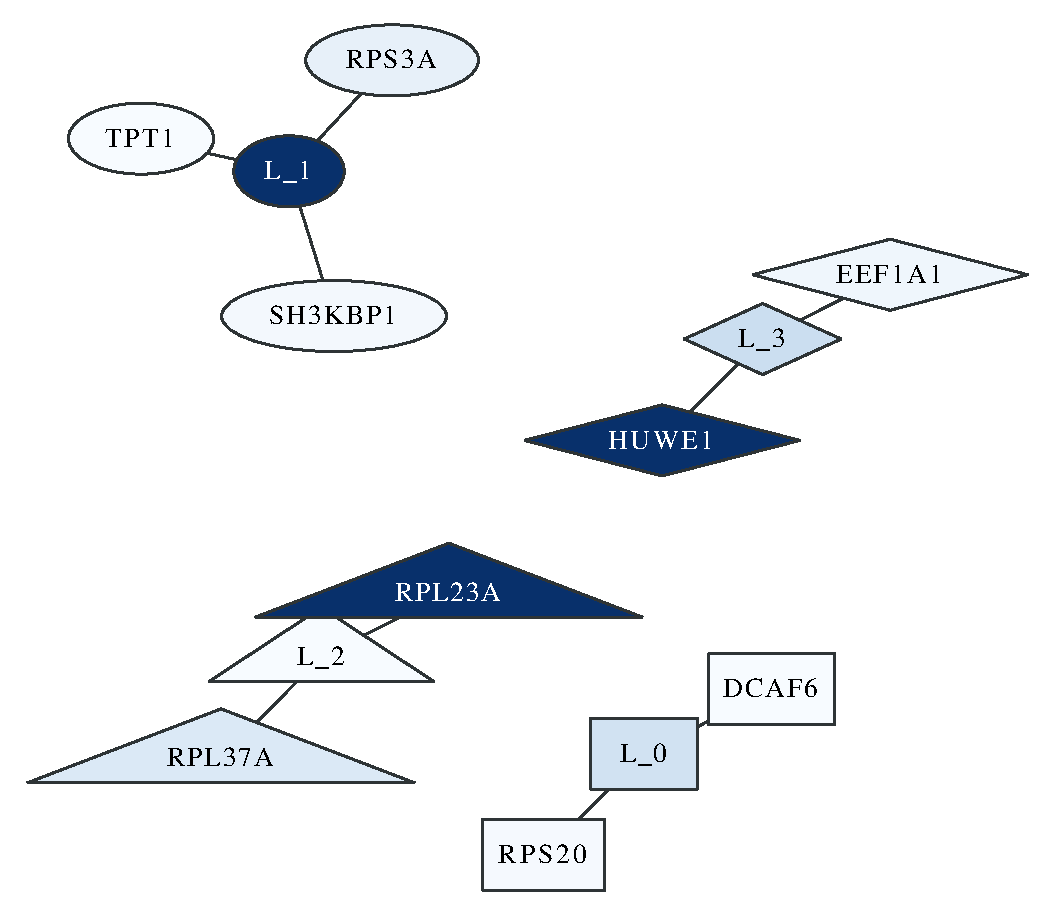
\includegraphics[width=0.49\textwidth]{figs/rat/figs/testdata-model-TCGA-LAML-GeneExpression-risk_group-4}}}\ \ 
  \subfigure[loose][]{\fbox{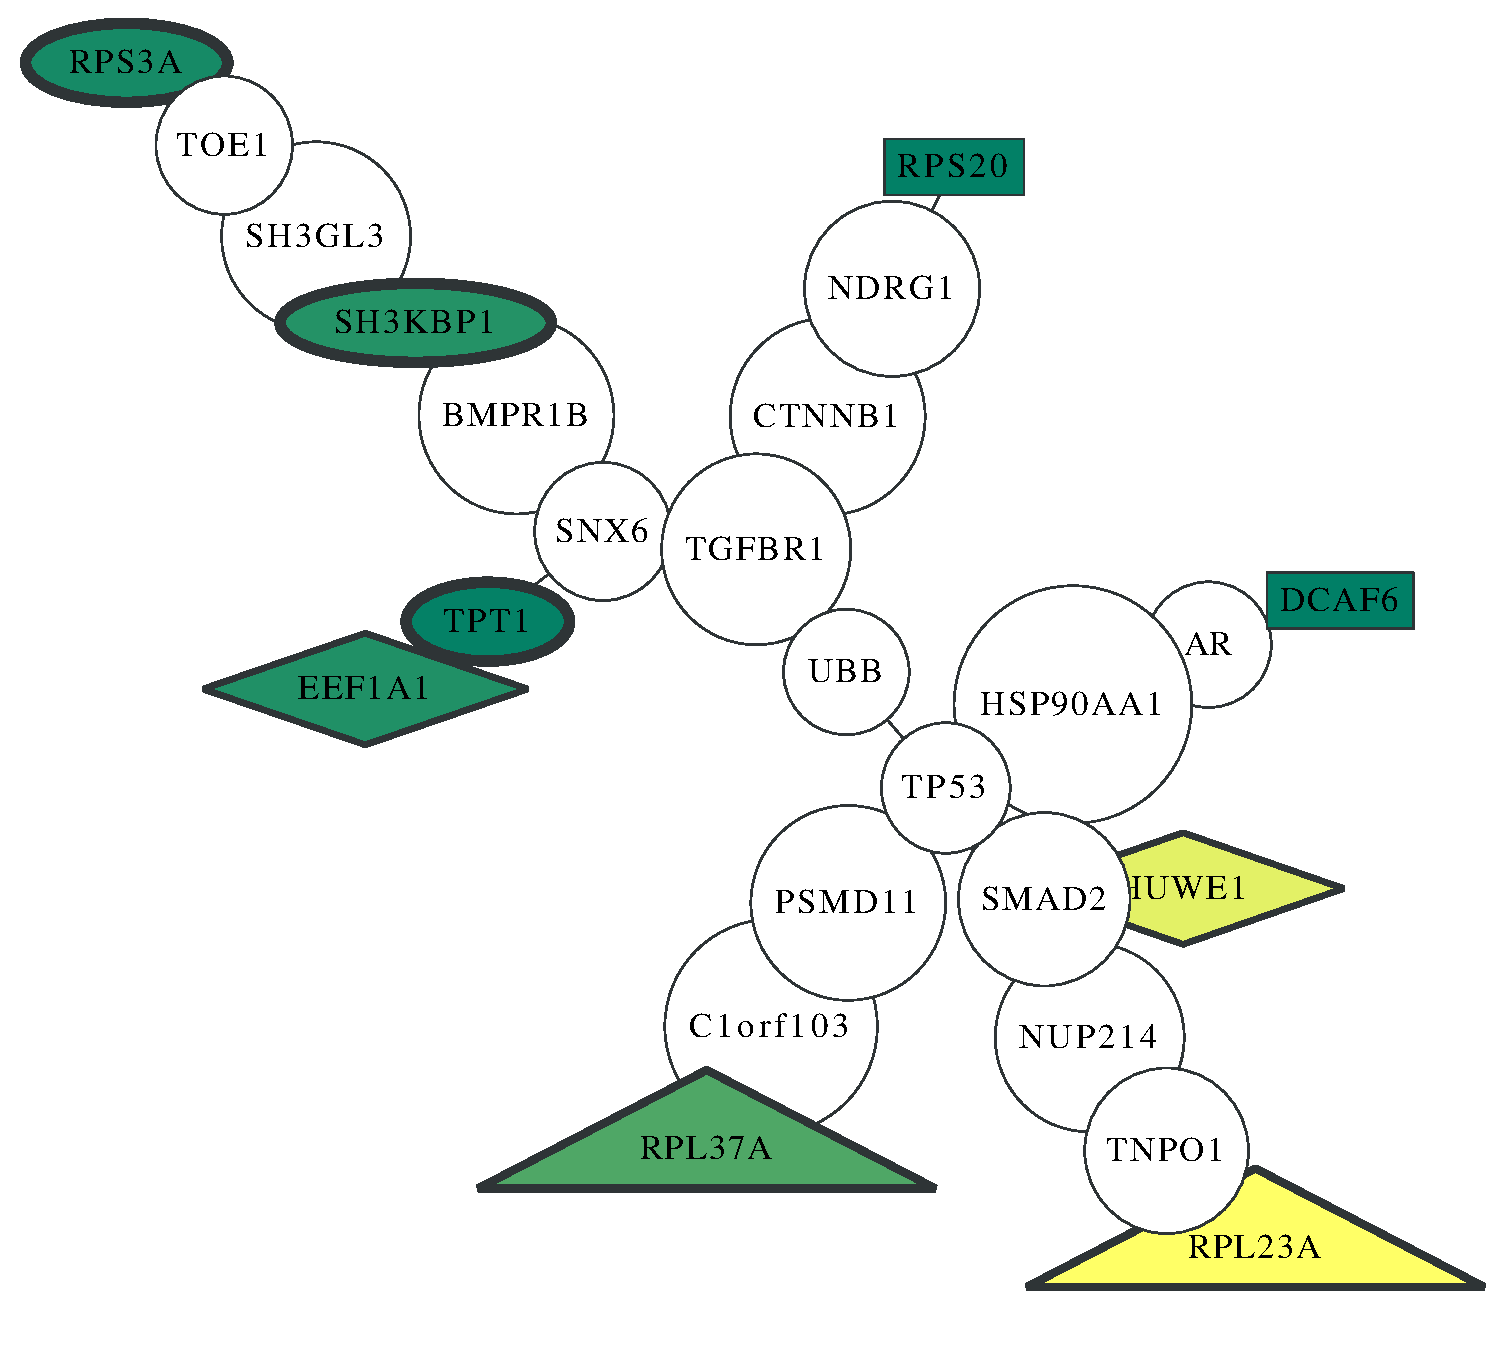
\includegraphics[width=0.49\textwidth]{figs/rat/figs/testdata-features-PPI-TCGA-LAML-GeneExpression-risk_group-4}}}
  \caption{\textbf{Visualization of one model} A sample model for TCGA-LAML gene expression data \textbf{(a)} individual classifiers and their selected features; higher confidence of a node is shown by a darker color, \textbf{(b)} selected genes plotted over the PPI network; green and yellow show low and high confidence respectively, and the thickness of the border of the node shows the respective confidence of the individual classifier to which it belongs.}
  \label{fig:sample-model}
\end{figure*}

To get a better overview of the individual features that were chosen by the classifiers for the particular test sample, we visualized the corresponding genes on a graph containing information about the PPI network in Fig.~\ref{fig:sample-model}(b). We extracted the PPI information from HPRD as explained before. This way, it is possible to find over- or under-regulated pathways that might be responsible for the label (e.g., cancer stage) of the test sample. Since PPI networks can be quite dense, we removed parts of the induced network. For this purpose we computed each shortest path between all pairs of selected features. Then, the minimum spanning tree of that section was plotted, after removing branches with no selected feature.

Most of the features chosen by any of the classifiers (colored nodes) are not connected to any other chosen feature. It is known that there is in many cases a correlation between expression value of the genes whose corresponding proteins interact~\cite{jansen2002relating}.
Therefore, a regularized model will only choose a subset of the correlated features. This explains the observation that features selected by a single model can be distant from each other on a PPI network; but if multiple disjoint sparse models are fit to the data, their selected features might happen to be close to each other on the PPI network (e.g., node TPT1 and node EEF1A1 in Fig.~\ref{fig:sample-model}(b)).

It is worth noting that these plots are the result of analyzing one single given test sample. Therefore in practice, these interpretations can be used for each patient and if useful, influence the treatment that the oncologist prescribe for the patient.


\textbf{Visualization of Important Global Features:}
As explained in Section~\ref{sec:visualization-of-model-predictions}, a graph is created from model structures of all 100 random training partitions, and then it is pruned to keep only high confidence nodes and edges.
The density estimation of the graph edge weights and the pruned graph are plotted in Fig.~\ref{fig:summary-network} where the nodes with labels are the ones that are not pruned. The nodes in this figure that do not have any label, are the ones with frequency lower than the corresponding threshold. Among the features considered to be important were features that had previously been linked to leukemia such as SH3KBP1~\cite{Adelaide2010}.

\begin{figure*}[!htpb]
\setlength{\fboxsep}{0pt}%
\setlength{\fboxrule}{0.5pt}%
  \subfigure[loose][]{\fbox{\includegraphics[width=0.49\textwidth]{figs/rat/figs/density-TCGA-LAML-GeneExpression-risk_group-2}}}\ \
  \subfigure[loose][]{\fbox{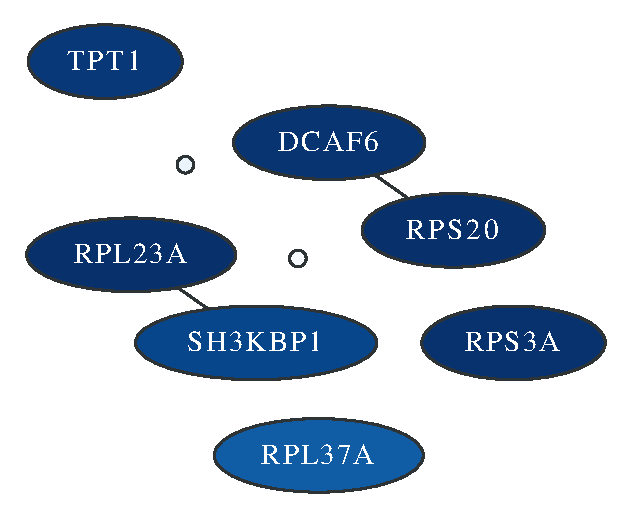
\includegraphics[width=0.49\textwidth]{figs/rat/figs/summary-TCGA-LAML-GeneExpression-risk_group-02}}}
  \caption{\textbf{(a) Determine pruning threshold} Threshold is determined by finding the point after which, $90\%$ of the area under the curve is observed from left to right. The horizontal axis shows the observed frequency or weight of the edges. \textbf{(b) Important Global Features} High confidence nodes and edges of the graph generated from the model on TCGA-LAML gene expression data. Darker color represents higher rate of being selected by a classifier.}
  \label{fig:summary-network}
\end{figure*}

What was more intriguing to see was that four out of the seven important features of the TCGA-LAML gene expression data set contained ribosomal proteins when using the risk group label, i.e. RPL37A, RPS20, RPS3A, and RPL23A. For a long time ribosomes were just considered machines that perform an unbiased translation of genes from mRNA to amino acid sequences, but this view has recently been challenged~\cite{Xue2012}. One new hypothesis is that the ribosome introduces an additional regulatory layer. Therefore, it could very well be that mutations in ribosomal proteins can lead to a misregulation of expression levels of important genes and ultimately to the development of cancer (in this case leukemia). One of the ribosomal proteins we found was RPL23A. It has been shown that loss of RPL23A can impede growth and lead to morphological abnormalities in Arabidopsis Thaliana~\cite{Xue2012}. Therefore, a mutation in RPL23A might also have severe effects in humans. A missense mutation in RPL23A was recently found in patients having Diamond-Blackfan anemia, which is an inherited form of pure red cell aplasia (related to leukemia)~\cite{Gazda2012}. Note that the model for LAML has low performance for the regularization value chosen. Nevertheless, the features shown here are also the ones with the highest confidence for models learnt with less regularization (with several other additional features). The models with less regularization show similar performance to the other methods shown in Fig.~\ref{fig:performance-summary}

\subsubsection{Performance comparison}
The performance of the method was compared with that of two ensemble methods, AdaBoost and stochastic gradient boosting, as well as an SVM with linear kernel, and an SVM with an RBF kernel. We also included our implementation of the NICK method~\cite{Lavi2012}.
We randomly partitioned the data into training and test sets with $80\%$ of the data for training and $20\%$ of the data for testing. To compare the performance of the different methods, Area Under the receiver operating characteristic Curve (AUC)~\cite{egan1975signal} was calculated on the test set over the decision values returned by the methods on the individual samples. The process was repeated 100 times to reduce random effects.
As seen in Fig.~\ref{fig:performance-summary}, overall performances of all methods are comparable. In some cases a single SVM works better, in some other cases ensemble algorithms give a better performance. However, in most cases an improvement in performance is observed by adding individual learners to the model, with the greatest gains due to the first few individual learners added to the model. 
In two cases, TCGA-LAML/Vital status and TCGA-LAML/Risk Group, our
reported performance measures are significantly lower than other
methods. This, however, comes from the fact that we have enforced
extreme sparsity measures. The performance of the method increases and
reaches the other methods' performance levels if this constraint is
relaxed, as reported in supplementary 1. 
We enforced those sparsity measures for all models to avoid over-fitting. Optimizing the sparsity constraint via cross-validation would have been computationally expensive, which is why we preferred to be conservative. Had we optimized the sparsity constraint, we would have still been able to find the significant features while having similar performance as the other methods.


\begin{landscape}
\begin{figure*}[!th]
\centerline{\includegraphics[angle=270,width=15.7cm]{figs/rat/figs/performance}}
\caption{\textbf{Performance Summary (AUC)} Each box shows a $25$--$75\%$ interval, as well as the median, which is shown as a horizontal line in each box.}\label{fig:performance-summary}
\end{figure*}
\end{landscape}

\subsection{Conclusions}

Machine learning has become more and more popular in many real world scenarios for making sense of large collections of facts. Differences between the data used for training the method and new data for which the label should be predicted can limit the performance of prediction methods on those data. In this work we introduced a method that estimates these potential partial biases and incorporates them into the prediction function. We applied it to gene expression and DNA methylation measurements from cancer patients. Our method has state-of-the-art performance on many different prediction tasks. Furthermore, we show how to make sense of the predictions. Visualizing the important genes can lead to new biological insights, as shown for the TCGA-LAML data set with the risk group label. Instead of mapping the genes to PPI networks, one could also think of mapping them to signaling pathways~\cite{Kanehisa2014}.

Recently, a study showed that most published signatures are not significantly more associated with cancer outcome than random signatures~\cite{Venet2011}. One of the reasons for this finding is that the data comes from slightly different underlying hidden data distributions. Since our new method estimates this bias and corrects for it by up-weighting the classifiers that have higher confidence, we expect that it should be less susceptible to such differences in the data.

In this work we designed and developed a method that besides being a predictive model, it can be used for two different purposes. It can be used as an exploratory method to reveal potential features used in future studies; and it can be used to different underlying causes of the same disease and with its interpretability help oncologists to choose the treatment accordingly.

We would like to point out that the applicability of our method is not limited to cancer outcome prediction, and it can apply to many more scenarios. The method assumes that the data has enough features to select from, and that there are related features to those selected ones that can be used to estimate their reliability. These are conditions that almost all biological data satisfy, hence the method can be applied to them.

The method also works as a skeleton whose components can be easily
substituted. For example, by changing the classifier used in
individual learners to a multi-class classifier, the method would work
on multi-class problems. For the sake of simplicity and without loss
of generality we performed the evaluations only on binary
classification problems. Also, due to the structure of our model, one possible approach would be to use a method such as iRDA and use those gene sets as features of individual learners. Whether this approach leads to better results or not requires further research.
Also, the combination of maximal information coefficient and Gaussian
processes is not the only feasible option, and they can be replaced
with other faster methods if the time complexity of the method is of
any concern. Some of these alternatives are already available on the
\emph{github} repository of the method.


\section{Raccoon}


\chapter{Conclusion}
In chapter~\ref{sec:fcs} we covered a flow cytometry data analysis pipeline, and
its application to two types of non-Hodgkin lymphoma, \emph{i.e.} Follicular
Lymphoma and Diffuse Large B Cell Lymphomas. We showed how the pipeline can
extract novel insights from the data as well as effectively automate a laborious
workflow.

We showed how flowType can extract features which can be used to train a model
to classify subtypes. However, we did not consider the relationships between
those features, \emph{i.e.} cell populations, while training the model. One
approach would be to design a kernel which takes into account those
relationships and therefore implicitly reduce the dimensionality of the input
data.

In chapter~\ref{sec:adaptive-learning} we focused mostly on the analysis of DNA
methylation data using adaptive and interpretable models. Although we put a
heavy focus on the models, our experiments showed that the preprocessing step
can play a crucial role in stability and the performance of those models. In the
case of DNA methylation data, for instance, a step to aggregate methylation
levels over genes made the models more stable, faster, and better performing.
Our observations support the idea of putting more focus on the preprocessing
steps, and to document them in a more informative way. This would also greatly
help towards improved reproducibility of efforts in the field.


\backmatter
\appendix
\chapter{RchyOptimyx Appendix}
\begin{table}[ht]\footnotesize
  \begin{center}
    \caption{The phenotypes with a high overlap with the BCR(pBLNK)$^+$ compartment as identified by flowType. The table includes the cell proportion of these immunophenotypes (second column) and the differences in the cell proportion of BCR(pBLNK)$^+$ cells in the stimulated and unstimulated assays (third column).}
    \label{apx:BCR}
    \begin{tabular}{lll}
      \hline
      Phenotype Name & Cell Proportion & BCR$^+_{(stim-unstim)}$ \\ 
      \hline
      CD19+CD4-CD8-CD34+CD20+CD123+CD38-CD3- & 0.001 & 0.160 \\ 
      CD19+CD4-CD34+CD20+CD123+CD38-CD3- & 0.001 & 0.160 \\ 
      CD19+CD4-CD34+CD20+CD123+CD3- & 0.001 & 0.155 \\ 
      \hline
    \end{tabular}
  \end{center}
\end{table}

% latex table generated in R 2.14.1 by xtable 1.7-0 package
% Mon Mar 19 12:59:47 2012
\begin{table}[ht]\footnotesize
  \begin{center}
    \caption{The phenotypes with a high overlap with the IL7(pSTAT5)$^+$ compartment as identified by flowType. The table includes the cell proportion of these immunophenotypes (second column) and differences in the cell proportion of IL7(pSTAT5)$^+$ cells in the stimulated and unstimulated assays (third column).}
    \label{apx:IL7}
    \begin{tabular}{lll}
      \hline
      Phenotype Name & Cell Proportion & IL7$^+_{(stim-unstim)}$ \\ 
      \hline
        CD19-CD4+CD8+CD20+CD33+CD38-CD3+ & 0.008 & 0.364 \\ 
        CD19-CD4+CD8+CD20+CD33+CD3+ & 0.008 & 0.366 \\ 
        CD19-CD4+CD8+CD34+CD33+CD38-CD3+ & 0.008 & 0.366 \\ 
        CD19-CD4+CD8+CD34+CD33+CD3+ & 0.008 & 0.368 \\ 
        CD19-CD4+CD8+CD34+CD20+CD33+CD38-CD3+ & 0.006 & 0.399 \\ 
        CD19-CD4+CD8+CD34+CD20+CD33+CD3+ & 0.006 & 0.402 \\ 
        CD4+CD8+CD20+CD33+CD38-CD3+ & 0.011 & 0.365 \\ 
        CD4+CD8+CD20+CD33+CD3+ & 0.011 & 0.371 \\ 
        CD4+CD8+CD34+CD33+CD38-CD3+ & 0.011 & 0.366 \\ 
        CD4+CD8+CD34+CD33+CD3+ & 0.011 & 0.371 \\ 
        CD4+CD8+CD34+CD20+CD33+CD38-CD3+ & 0.008 & 0.399 \\ 
        CD4+CD8+CD34+CD20+CD33+CD3+ & 0.009 & 0.405 \\ 
        CD19+CD4+CD8+CD20+CD33+CD38-CD3+ & 0.003 & 0.364 \\ 
        CD19+CD4+CD8+CD20+CD33+CD3+ & 0.003 & 0.378 \\ 
        CD19+CD4+CD8+CD34+CD33+CD38-CD3+ & 0.003 & 0.359 \\ 
        CD19+CD4+CD8+CD34+CD33+CD3+ & 0.003 & 0.372 \\ 
        CD19+CD4+CD8+CD34+CD20+CD33+CD38-CD3+ & 0.002 & 0.397 \\ 
        CD19+CD4+CD8+CD34+CD20+CD33+CD3+ & 0.002 & 0.409 \\ 
      \hline
    \end{tabular}
  \end{center}
\end{table}


% latex table generated in R 2.14.1 by xtable 1.7-0 package
% Mon Mar 19 12:55:05 2012
\begin{table}[ht]\footnotesize
  \begin{center}
    \caption{The phenotypes with a high overlap with the LPS(p-p38)$^+$ compartment as identified by flowType. The table includes the cell proportion of these immunophenotypes (second column) and differences in the cell proportion of LPS(p-p38)$^+$ cells in the stimulated and unstimulated assays (third column).}
    \label{apx:LPS}
    \begin{tabular}{lll}
      \hline
      Phenotype Name & Cell Proportion & LPS$^+_{(stim-unstim)}$ \\ 
      \hline
      CD19-CD4-CD8-CD34-CD20-CD33+CD123-CD38-CD3- & 0.008 & 0.474 \\ 
      CD19-CD4-CD8-CD34-CD20-CD33+CD123-CD3- & 0.008 & 0.473 \\ 
      CD19-CD4-CD8-CD34-CD20-CD33+CD38-CD3- & 0.009 & 0.466 \\ 
      CD19-CD4-CD8-CD34-CD20-CD33+CD3- & 0.009 & 0.465 \\ 
      CD19-CD4-CD8-CD34-CD33+CD123-CD38-CD3- & 0.022 & 0.460 \\ 
      CD19-CD4-CD8-CD34-CD33+CD123-CD3- & 0.022 & 0.459 \\ 
      CD19-CD4-CD8-CD34-CD33+CD38-CD3- & 0.022 & 0.452 \\ 
      CD19-CD4-CD8-CD34-CD33+CD3- & 0.022 & 0.451 \\ 
      CD19-CD4-CD8-CD34-CD20+CD33+CD123-CD38-CD3- & 0.013 & 0.450 \\ 
      CD19-CD4-CD8-CD34-CD20+CD33+CD123-CD3- & 0.013 & 0.449 \\ 
      CD19-CD4-CD8-CD20-CD33+CD123-CD38-CD3- & 0.023 & 0.453 \\ 
      CD19-CD4-CD8-CD20-CD33+CD123-CD3- & 0.023 & 0.452 \\ 
      CD19-CD4-CD34-CD20-CD33+CD123-CD38-CD3- & 0.011 & 0.456 \\ 
      CD19-CD4-CD34-CD20-CD33+CD123-CD3- & 0.011 & 0.455 \\ 
      CD19-CD8-CD34-CD20-CD33+CD123-CD38-CD3- & 0.012 & 0.462 \\ 
      CD19-CD8-CD34-CD20-CD33+CD123-CD3- & 0.012 & 0.461 \\ 
      CD19-CD8-CD34-CD20-CD33+CD38-CD3- & 0.012 & 0.454 \\ 
      CD19-CD8-CD34-CD20-CD33+CD3- & 0.012 & 0.454 \\ 
      CD4-CD8-CD34-CD20-CD33+CD123-CD38-CD3- & 0.011 & 0.462 \\ 
      CD4-CD8-CD34-CD20-CD33+CD123-CD3- & 0.011 & 0.461 \\ 
      CD4-CD8-CD34-CD20-CD33+CD38-CD3- & 0.011 & 0.454 \\ 
      CD4-CD8-CD34-CD20-CD33+CD3- & 0.011 & 0.454 \\ 
      CD8-CD34-CD20-CD33+CD123-CD38-CD3- & 0.015 & 0.450 \\ 
      CD8-CD34-CD20-CD33+CD123-CD3- & 0.015 & 0.449 \\ 
      \hline
    \end{tabular}
  \end{center}
\end{table}

% latex table generated in R 2.11.1 by xtable 1.5-6 package
% Sat Dec 11 12:28:36 2010
% \begin{table}\tiny
\begin{landscape}
\begin{center}
  {\tiny 
    % \begin{longtable}{rp{6cm}lllll}
    \begin{longtable}{rlllllll}
      \caption{\normalsize Statistically significant immunophenotypic correlates of survival of HIV$^+$ subjects are predicted by flowType. The p-values of the log rank tests, 95\% confidence intervals calculated using bootstrapping, adjusted p-values using Bonferroni's method, coefficients and $R^2$ values of the Cox proportional hazards regression models, and the frequency of the cells are provided as columns of the table.}\\
 \hline
      \# & Phenotype & p-value & p-value, CI & adjusted & CPHR & R$^2$ & Cell \\
      &  & & & p-value & Coefficient &  & Frequency \\
      \hline
      \endhead
      1 & CD28-CD45RO+CD57-CCR5+ & 5.3e-07 & (4.3e-14, 1.3e-02) & 2e-02 &  20.5 & 0.056 & 0.03048 \\ 
      2 & CD28-CD8+CD57-CD127- & 2.5e-07 & (2.3e-14, 3.8e-04) & 1e-02 &  12.3 & 0.060 & 0.05975 \\ 
      3 & CD28-CD45RO+CD57-CCR7- & 5.1e-07 & (2.3e-14, 6.1e-04) & 2e-02 &  15.7 & 0.057 & 0.03829 \\ 
      4 & CD28-CD45RO+CD4-CD57- & 3.5e-07 & (2.3e-14, 1.1e-03) & 1e-02 &  13.2 & 0.058 & 0.04357 \\ 
      5 & CD45RO+CD4-CD57-CD127- & 2.7e-07 & (1.2e-13, 7.1e-03) & 1e-02 &  12.8 & 0.059 & 0.05062 \\ 
      6 & CD28-CD45RO+CD57-CD127- & 4.7e-08 & (1.7e-14, 6.8e-04) & 2e-03 &  16.0 & 0.067 & 0.03732 \\ 
      7 & CD45RO+CD4-CD27-CD127- & 4.4e-07 & (5.8e-14, 1.1e-03) & 2e-02 &  14.3 & 0.057 & 0.04830 \\ 
      8 & CD28-CD45RO+CD57- & 5.6e-07 & (4.4e-14, 4.1e-04) & 2e-02 &  12.4 & 0.056 & 0.05015 \\ 
      9 & CD45RO+CD4-CD127- & 6.5e-07 & (4.7e-15, 2.9e-03) & 2e-02 &   9.6 & 0.056 & 0.07176 \\ 
      10 & CD28-CD45RO+CD4-CD127- & 3.1e-07 & (0.0e+00, 5.7e-03) & 1e-02 &  11.7 & 0.059 & 0.05300 \\ 
      11 & CD28-CD45RO+CD57-CCR5+CD27-CCR7+CD127- & 4.7e-07 & (5.7e-14, 7.7e-03) & 2e-02 & 171.4 & 0.057 & 0.00315 \\ 
      12 & CD28-CD45RO+CD4-CD57-CCR5+CD27-CCR7+CD127- & 4.5e-07 & (1.8e-13, 3.9e-04) & 2e-02 & 176.2 & 0.057 & 0.00294 \\ 
      13 & CD28-CD57-CD127- & 3.3e-07 & (3.4e-15, 8.0e-03) & 1e-02 &   8.0 & 0.058 & 0.12341 \\ 
      14 & CD28-CD4-CD57- & 8.8e-07 & (2.2e-15, 2.9e-03) & 3e-02 &   7.2 & 0.054 & 0.15525 \\ 
      15 & CD57-CD27-CD127- & 6.2e-08 & (2.4e-14, 4.7e-03) & 2e-03 &   9.5 & 0.065 & 0.12173 \\ 
      16 & CD4-CD57-CD27-CD127- & 4.7e-08 & (4.2e-14, 3.3e-03) & 2e-03 &   9.7 & 0.067 & 0.09721 \\ 
      17 & CD28-CD57-CCR7-CD127- & 2.8e-07 & (9.7e-15, 1.0e-02) & 1e-02 &   9.8 & 0.059 & 0.08417 \\ 
      18 & CD28-CD4-CD57-CD127- & 3.3e-08 & (2.0e-12, 5.7e-04) & 1e-03 &   9.1 & 0.068 & 0.10852 \\ 
      19 & CD4-CD57-CCR7-CD127- & 6.5e-07 & (3.8e-15, 2.3e-03) & 2e-02 &   8.8 & 0.056 & 0.09501 \\ 
      20 & CD45RO-CD4-CD57+CCR5-CD27+CCR7-CD127- & 6.1e-07 & (1.2e-12, 2.6e-03) & 2e-02 & 498.4 & 0.056 & 0.00097 \\ 
      21 & CD28-CD45RO-CD4-CD57+CCR5-CD27+CCR7-CD127- & 2.5e-07 & (0.0e+00, 7.7e-03) & 1e-02 & 561.2 & 0.060 & 0.00074 \\ 
      22 & CD45RO-CD8+CD57+CCR5-CD27+CCR7-CD127- & 1.2e-07 & (4.6e-14, 3.3e-04) & 5e-03 & 638.6 & 0.063 & 0.00068 \\ 
      23 & CD45RO-CD8+CD4-CD57+CCR5-CD27+CCR7-CD127- & 1.2e-07 & (5.1e-14, 2.0e-03) & 5e-03 & 638.6 & 0.063 & 0.00068 \\ 
      24 & CD28-CD45RO-CD4-CD57+CCR5-CD27+CD127- & 5.7e-07 & (1.1e-13, 2.3e-03) & 2e-02 & 298.3 & 0.056 & 0.00099 \\ 
      25 & KI-67+CD28-CCR5+ & 1.0e-11 & (2.9e-13, 2.8e-03) & 4e-07 &  96.1 & 0.101 & 0.00547 \\ 
      26 & KI-67+CD28-CCR5+CD27- & 8.7e-12 & (1.5e-14, 8.9e-04) & 3e-07 & 115.3 & 0.102 & 0.00453 \\ 
      27 & KI-67+CCR5+ & 1.3e-11 & (2.4e-14, 7.0e-03) & 5e-07 &  53.4 & 0.100 & 0.01192 \\ 
      28 & KI-67+CD28+CD45RO+CD57-CCR7-CD127- & 4.2e-09 & (5.6e-16, 3.0e-03) & 2e-04 & 241.3 & 0.077 & 0.00209 \\ 
      29 & KI-67+CD45RO-CD4-CD27-CCR7-CD127- & 1.2e-09 & (2.0e-14, 4.4e-03) & 4e-05 & 161.9 & 0.082 & 0.00297 \\ 
      30 & KI-67+CD28-CD45RO-CD8-CD4- & 5.0e-09 & (2.9e-12, 1.7e-03) & 2e-04 & 176.0 & 0.076 & 0.00225 \\ 
      31 & KI-67+CD8-CD4- & 8.1e-09 & (6.1e-13, 4.5e-02) & 3e-04 &  58.1 & 0.074 & 0.00738 \\ 
      32 & KI-67+CCR5+CD27-CCR7- & 2.0e-11 & (3.8e-14, 6.0e-04) & 8e-07 & 109.8 & 0.099 & 0.00532 \\ 
      33 & KI-67+CD8-CCR5+CCR7- & 1.3e-10 & (3.1e-13, 2.0e-03) & 5e-06 & 147.3 & 0.091 & 0.00392 \\ 
      34 & KI-67+CD28-CD8-CCR5+CCR7+CD127- & 2.6e-09 & (1.6e-14, 1.1e-02) & 1e-04 & 625.8 & 0.079 & 0.00061 \\ 
      35 & KI-67+CD28+CD45RO+CD8+CD57-CD27+CCR7+ & 6.7e-07 & (3.8e-13, 1.5e-03) & 3e-02 & 585.4 & 0.055 & 0.00051 \\ 
      36 & KI-67+CD28+CD45RO+CD8+CD4-CD57-CD27+CCR7+ & 6.7e-07 & (1.1e-16, 4.7e-03) & 3e-02 & 585.4 & 0.055 & 0.00051 \\ 
      37 & KI-67+CD8+CD27-CCR7-CD127- & 4.7e-11 & (1.3e-13, 1.4e-03) & 2e-06 & 141.3 & 0.095 & 0.00292 \\ 
      38 & KI-67+CD8+CD4-CD27-CCR7-CD127- & 4.7e-11 & (1.3e-13, 1.3e-03) & 2e-06 & 141.3 & 0.095 & 0.00292 \\ 
      39 & KI-67+CD28-CD8+CD27-CCR7-CD127- & 2.7e-11 & (1.0e-13, 7.6e-04) & 1e-06 & 164.5 & 0.097 & 0.00241 \\ 
      40 & KI-67+CD28-CD8+CD4-CD27-CCR7-CD127- & 2.7e-11 & (2.7e-13, 1.4e-03) & 1e-06 & 164.5 & 0.097 & 0.00241 \\ 
      41 & KI-67+CD28-CD8+CCR7-CD127- & 6.6e-11 & (5.6e-14, 1.5e-02) & 3e-06 & 132.9 & 0.094 & 0.00293 \\ 
      42 & KI-67+CD28-CD8+CD4-CCR7-CD127- & 6.6e-11 & (1.2e-14, 8.4e-04) & 3e-06 & 132.9 & 0.094 & 0.00293 \\ 
      43 & KI-67+CD45RO+CD8+CD27-CCR7- & 1.2e-09 & (4.0e-12, 2.8e-03) & 5e-05 & 143.6 & 0.082 & 0.00216 \\ 
      44 & KI-67+CD45RO+CD8+CD4-CD27-CCR7- & 1.2e-09 & (1.0e-12, 1.2e-02) & 5e-05 & 143.6 & 0.082 & 0.00216 \\ 
      45 & KI-67+CD28-CD45RO+CD8+CD27-CCR7- & 1.0e-09 & (1.9e-15, 7.3e-04) & 4e-05 & 188.5 & 0.082 & 0.00155 \\ 
      46 & KI-67+CD28-CD45RO+CD8+CD4-CD27-CCR7- & 1.0e-09 & (1.7e-13, 2.0e-03) & 4e-05 & 188.5 & 0.082 & 0.00155 \\ 
      47 & KI-67+CD45RO+CD8+CD27-CD127- & 7.1e-10 & (1.2e-14, 6.8e-03) & 3e-05 & 152.4 & 0.084 & 0.00221 \\ 
      48 & KI-67+CD45RO+CD8+CD4-CD27-CD127- & 7.1e-10 & (3.4e-14, 1.5e-03) & 3e-05 & 152.4 & 0.084 & 0.00221 \\ 
      49 & KI-67+CD28-CD45RO+CD8+CD27-CD127- & 5.0e-10 & (6.0e-13, 3.1e-03) & 2e-05 & 201.3 & 0.085 & 0.00163 \\ 
      50 & KI-67+CD28-CD45RO+CD8+CD4-CD27-CD127- & 5.0e-10 & (4.6e-14, 2.7e-03) & 2e-05 & 201.3 & 0.085 & 0.00163 \\ 
      51 & KI-67+CD28-CD45RO+CD8+CD127- & 1.0e-09 & (1.2e-15, 3.2e-03) & 4e-05 & 150.5 & 0.083 & 0.00222 \\ 
      52 & KI-67+CD28-CD45RO+CD8+CD4-CD127- & 1.0e-09 & (1.5e-11, 3.6e-03) & 4e-05 & 150.5 & 0.083 & 0.00222 \\ 
      53 & KI-67+CD45RO+CD8+CD4-CD127- & 2.2e-09 & (2.8e-13, 2.1e-03) & 9e-05 &  99.8 & 0.079 & 0.00362 \\ 
      54 & KI-67+CD28-CD45RO+CD8+CD4-CCR7- & 8.0e-09 & (2.7e-12, 7.2e-04) & 3e-04 & 133.6 & 0.074 & 0.00209 \\ 
      55 & KI-67+CD28-CD45RO+CD57-CCR7+CD127- & 5.9e-08 & (4.0e-15, 4.5e-03) & 2e-03 & 376.6 & 0.066 & 0.00075 \\ 
      56 & KI-67+CD28-CD45RO+CD4-CD57-CCR7+CD127- & 5.0e-08 & (4.8e-13, 3.9e-03) & 2e-03 & 409.6 & 0.066 & 0.00070 \\ 
      57 & KI-67+CD57-CD27-CD127- & 5.9e-10 & (3.2e-14, 2.7e-03) & 2e-05 &  44.9 & 0.085 & 0.00806 \\ 
      58 & KI-67+CD28-CD27-CD127- & 4.8e-10 & (7.3e-15, 2.5e-03) & 2e-05 &  50.6 & 0.086 & 0.00711 \\ 
      59 & KI-67+CD4-CD127- & 1.3e-10 & (4.4e-16, 9.7e-03) & 5e-06 &  37.1 & 0.091 & 0.01159 \\ 
      60 & KI-67+CD28-CD127- & 4.9e-10 & (1.1e-12, 1.4e-03) & 2e-05 &  41.4 & 0.086 & 0.00823 \\ 
      61 & KI-67+CD4-CD27- & 5.6e-09 & (2.1e-14, 2.6e-03) & 2e-04 &  28.6 & 0.075 & 0.01122 \\ 
      62 & KI-67+CD28-CD4-CD27- & 1.8e-09 & (3.6e-13, 5.3e-03) & 7e-05 &  40.2 & 0.080 & 0.00785 \\ 
      63 & KI-67+CD27-CD127- & 1.3e-09 & (9.8e-15, 1.1e-03) & 5e-05 &  33.0 & 0.082 & 0.01052 \\ 
      64 & KI-67+CCR7-CD127- & 6.5e-11 & (1.4e-15, 9.6e-04) & 2e-06 &  47.3 & 0.094 & 0.00947 \\ 
      65 & KI-67+CD4-CD27-CCR7- & 9.6e-11 & (1.1e-16, 1.5e-03) & 4e-06 &  52.1 & 0.092 & 0.00764 \\ 
      66 & KI-67+CD4-CCR7- & 1.7e-10 & (3.0e-14, 1.0e-02) & 7e-06 &  41.4 & 0.090 & 0.00987 \\ 
      67 & KI-67+CD45RO+CD57-CCR7- & 1.4e-09 & (6.6e-13, 1.2e-03) & 5e-05 &  49.6 & 0.081 & 0.00695 \\ 
      68 & KI-67+CD45RO+CD57-CD27-CCR7- & 9.1e-10 & (8.6e-12, 2.5e-03) & 3e-05 &  66.4 & 0.083 & 0.00505 \\ 
      69 & KI-67+CD45RO+CD4- & 2.0e-09 & (8.0e-13, 2.5e-03) & 8e-05 &  45.3 & 0.080 & 0.00851 \\ 
      70 & KI-67+CD28-CD45RO+ & 1.3e-08 & (1.2e-12, 2.4e-03) & 5e-04 &  54.9 & 0.072 & 0.00525 \\ 
      71 & KI-67+CD45RO+CD127- & 1.1e-09 & (4.4e-16, 1.5e-02) & 4e-05 &  42.5 & 0.082 & 0.00834 \\ 
      72 & KI-67+CD45RO+CD57-CD127- & 2.9e-10 & (1.5e-14, 6.4e-04) & 1e-05 &  55.0 & 0.088 & 0.00719 \\ 
      73 & KI-67+CD28-CD45RO+CD8+CD27- & 9.2e-09 & (2.6e-15, 2.3e-03) & 4e-04 & 138.0 & 0.073 & 0.00201 \\ 
      74 & KI-67+CD28-CD45RO+CD8+CD4-CD27- & 9.2e-09 & (1.0e-15, 4.6e-03) & 4e-04 & 138.0 & 0.073 & 0.00201 \\ 
      75 & KI-67+CD8+CD4-CD57-CD27-CD127- & 1.9e-09 & (5.9e-14, 7.0e-03) & 7e-05 & 113.8 & 0.080 & 0.00274 \\ 
      76 & KI-67+CD28-CD45RO+CD8+ & 9.3e-09 & (5.9e-13, 1.4e-03) & 4e-04 & 102.7 & 0.073 & 0.00279 \\ 
      77 & KI-67+CD28-CD45RO+CD8+CD4- & 9.3e-09 & (0.0e+00, 1.6e-03) & 4e-04 & 102.7 & 0.073 & 0.00279 \\ 
      78 & KI-67+CD45RO+CD8+ & 2.1e-08 & (6.9e-15, 6.8e-04) & 8e-04 &  59.1 & 0.070 & 0.00512 \\ 
      79 & KI-67+CD8+CCR7- & 3.0e-08 & (7.7e-13, 2.8e-03) & 1e-03 &  49.5 & 0.068 & 0.00530 \\ 
      80 & KI-67+CD8+CD27-CCR7- & 8.3e-09 & (1.0e-13, 3.6e-03) & 3e-04 &  70.7 & 0.074 & 0.00377 \\ 
      81 & KI-67+CD4- & 2.8e-08 & (1.0e-13, 2.3e-03) & 1e-03 &  17.1 & 0.069 & 0.01627 \\ 
      82 & KI-67+CD28-CD4- & 1.1e-08 & (5.9e-14, 4.0e-03) & 4e-04 &  26.7 & 0.073 & 0.00950 \\ 
      83 & KI-67+CD127- & 2.7e-08 & (1.2e-12, 2.1e-03) & 1e-03 &  19.1 & 0.069 & 0.01460 \\ 
      84 & KI-67+CCR7- & 8.4e-08 & (3.4e-15, 2.3e-03) & 3e-03 &  18.3 & 0.064 & 0.01311 \\ 
      85 & KI-67+CD27-CCR7- & 3.5e-08 & (1.7e-13, 1.2e-03) & 1e-03 &  25.2 & 0.068 & 0.00998 \\ 
      86 & KI-67+CD45RO+CD27- & 7.5e-07 & (5.4e-13, 1.8e-03) & 3e-02 &  24.0 & 0.055 & 0.00862 \\ 
      87 & KI-67+CD45RO+CD57- & 1.2e-07 & (2.1e-13, 3.1e-03) & 5e-03 &  22.9 & 0.062 & 0.01123 \\ 
      88 & KI-67+CD4-CD57- & 1.3e-08 & (3.8e-15, 2.1e-03) & 5e-04 &  25.3 & 0.072 & 0.01209 \\ 
      89 & KI-67+CD28-CD4-CD57- & 9.7e-09 & (5.5e-12, 1.2e-03) & 4e-04 &  37.7 & 0.073 & 0.00698 \\ 
      90 & KI-67+CD57-CD127- & 3.3e-09 & (1.3e-13, 3.3e-03) & 1e-04 &  28.1 & 0.078 & 0.01128 \\ 
      91 & KI-67+CD45RO+CCR7- & 4.2e-09 & (7.8e-15, 2.5e-03) & 2e-04 &  37.5 & 0.077 & 0.00819 \\ 
      92 & KI-67+CD57-CCR7- & 2.7e-08 & (2.8e-13, 2.8e-03) & 1e-03 &  26.6 & 0.069 & 0.01008 \\ 
      93 & KI-67+CD57-CD27-CCR7- & 1.2e-08 & (4.9e-13, 2.6e-03) & 5e-04 &  36.8 & 0.072 & 0.00762 \\ 
      94 & KI-67+CD28-CCR7- & 3.3e-09 & (4.6e-14, 5.7e-03) & 1e-04 &  37.7 & 0.078 & 0.00739 \\ 
      95 & KI-67+CD28-CD27-CCR7- & 3.3e-09 & (2.6e-14, 6.5e-04) & 1e-04 &  43.0 & 0.078 & 0.00647 \\ 
      96 & KI-67+CD28- & 1.9e-07 & (4.0e-15, 2.7e-03) & 7e-03 &  18.3 & 0.061 & 0.01053 \\ 
      97 & KI-67+CD28-CD27- & 7.1e-08 & (1.5e-12, 8.6e-04) & 3e-03 &  26.3 & 0.065 & 0.00874 \\ 
      98 & KI-67+CD28-CD8- & 8.3e-08 & (5.5e-14, 2.5e-03) & 3e-03 &  44.2 & 0.064 & 0.00523 \\ 
      99 & KI-67+CD45RO+ & 8.9e-07 & (1.9e-13, 2.5e-03) & 3e-02 &  15.4 & 0.054 & 0.01343 \\ 
      100 & KI-67+CD8+CD57- & 1.1e-06 & (4.4e-14, 3.1e-03) & 4e-02 &  28.3 & 0.053 & 0.00648 \\ 
      101 & KI-67+CD8+CD27- & 6.4e-07 & (2.3e-14, 1.1e-02) & 2e-02 &  35.2 & 0.056 & 0.00560 \\ 
      \hline
      \label{apx:tsl}
      % \end{table}
    \end{longtable}
  }
\end{center}
\end{landscape}


%\chapter{Last note}

\listoftables
\listoffigures

\bibliographystyle{abbrv}
\bibliography{thesis}

\end{document}
